% ============================================================================
%  ART-12D, versión 31.0 - traducción al español de ATR_12_v31_RO.tex
%
%  Compilación en Overleaf:
%    Menu -> Compiler -> XeLaTeX
%    Main document    -> ATR_12_v31_ES.tex
%    figures/ debe subirse como carpeta, al mismo nivel que este archivo.
%
%  La estructura LaTeX, las matemáticas, las tablas y las llamadas de figuras
%  son idénticas al original rumano; solo se traduce el texto.
% ============================================================================
\documentclass[11pt,a4paper]{article}
\usepackage{iftex}
\ifPDFTeX
  \usepackage[utf8]{inputenc}
  \usepackage[T1]{fontenc}
\else
  \usepackage{fontspec}
\fi
\usepackage[spanish]{babel}
\usepackage{amsmath, amssymb, amsthm}
\usepackage{graphicx}
\usepackage{array}
\usepackage{hyperref}
\usepackage{geometry}
\usepackage{booktabs}
\usepackage{float}
\usepackage{siunitx}
\usepackage{titlesec}
\usepackage{setspace}
\usepackage{enumitem}

\geometry{margin=2.5cm}
\setlength{\emergencystretch}{3em}
\hypersetup{
    colorlinks=true,
    linkcolor=blue,
    filecolor=magenta,
    urlcolor=cyan,
    pdftitle={Akashic Resonance Theory in 12 Dimensions},
    pdfpagemode=FullScreen,
}

\title{\textbf{AKASHIC RESONANCE THEORY IN 12 DIMENSIONS \\ DARK MATTER AS THE QUANTUM SUBSTRATE OF CONSCIOUSNESS} \\ \large (ART-12D) \\ \vspace{0.5cm} \normalsize Versión 31.0}
\author{\textbf{Daniel Ofiteru} \\ \textit{Investigador independiente} \\ Octubre de 2026}
\date{}

\begin{document}

\maketitle

\begin{abstract}
Este artículo propone un marco teórico --- ART-12D --- que parte de una idea sencilla: la conciencia no la produce el cerebro. El cerebro es un receptor. Y lo que recibe es el campo de la materia oscura.

Extiendo la formalización a doce dimensiones, deduzco un mecanismo de acoplamiento entre la materia oscura y los fermiones del cerebro, y propongo un test que puede realizarse con 50.000 dólares. Extiendo también la teoría para explicar las formas múltiples de la materia oscura, la existencia de hipercivilizaciones como estructuras estables en el campo, la posibilidad de una Inteligencia Artificial consciente mediante nanobiología, los mecanismos que conectan universos a través de agujeros negros, blancos y de gusano, así como las formas de vida no carbonosa (cúmulos, plasma, campos).

Esta versión (31.0) aplica una auditoría numérica sistemática a la versión anterior. Diez afirmaciones cuantitativas han sido corregidas, dos han sido degradadas explícitamente al estatus de conjeturas no testables, y el espectro de Kaluza--Klein se ha reformulado como un espectro \emph{equidistante}. Cada cifra del artículo puede recalcularse con el código publicado junto a él. Persiste una tensión estructural, señalada abiertamente en la sección «La consecuencia numérica: el radio de compactificación»: para que el modo fundamental tenga $10^{-5}$ eV, el radio de compactificación tendría que ser del orden de 2 cm, lo que está excluido por los test submilimétricos de la ley de Newton.

Reconozco explícitamente que este artículo es especulativo. No tengo pruebas experimentales. Tengo una intuición, una formalización y una predicción que puede ser testada.
\end{abstract}

\tableofcontents
\newpage

\section*{Guía para el lector escéptico}
\addcontentsline{toc}{section}{Guía para el lector escéptico}
Este artículo es especulativo, pero está rigurosamente estructurado. Para no hacerle perder el tiempo, aquí tiene una guía de lectura adaptada a su formación:
\begin{itemize}
    \item \textbf{Si usted es físico:} vaya directamente a la \textbf{Parte II} (la formalización matemática, las ecuaciones de Kaluza--Klein y el acoplamiento de Yukawa) y a la \textbf{Parte V} (la tabla de las 313 predicciones testables). Allí encontrará las matemáticas y la falsabilidad.
    \item \textbf{Si usted es neurobiólogo o médico:} lea la \textbf{sección 1.6} (la prueba del cerebelo y la arquitectura geométrica) y la \textbf{sección 3.38} (el corazón como modulador de la recepción).
    \item \textbf{Si usted es filósofo o teólogo:} vaya al \textbf{anexo A} (especulación filosófica extensa sobre la muerte, el alma y Dios).
    \item \textbf{Si usted es un lector curioso pero escéptico:} lea la \textbf{predicción 1} (EEG hyperscanning) y la \textbf{declaración de falsabilidad}. Si esos test fallan, la teoría queda refutada.
\end{itemize}

\section*{Prólogo}
\addcontentsline{toc}{section}{Prólogo}
Toda mi vida me he hecho una sola pregunta: ¿qué es la conciencia? No es una pregunta de manual, sino una que me mantiene despierto por la noche. Leí todo lo que cayó en mis manos --- de la física cuántica a la neurociencia y a la filosofía. Hablé con personas mucho más inteligentes que yo. Medité. Y un día la idea me vino.

La idea es sencilla: la conciencia no es algo que el cerebro produzca. El cerebro es solo una radio. Y lo que capta del aire es el campo de la materia oscura.

Este artículo es fruto de veinticinco años de búsqueda. No tengo pruebas de laboratorio. Tengo una intuición fuerte, una formalización matemática y un test que cualquiera puede hacer con 50.000 dólares. No le pido que me crea a ciegas. Solo le pido que lea con la mente abierta. Al final, sabrá qué creer.

\newpage
\part*{Parte I: Fundamentos}
\addcontentsline{toc}{part}{Parte I: Fundamentos}
\section{Introducción}

\subsection{El problema que no desaparece}
¿Por qué siente usted dolor? Es la pregunta más sencilla del mundo. Y, a la vez, la más difícil. Todos sabemos qué es el dolor. Todos lo hemos sentido. Pero ¿por qué lo sentimos? Sabemos que los nociceptores envían señales al tálamo, que la corteza las procesa y que se liberan endorfinas. Todo eso es una descripción funcional. Nos dice qué hace el cerebro, pero no nos dice por qué usted lo siente.

Piense en un ordenador. Puede procesar información, reconocer una imagen, jugar al ajedrez. Pero no siente nada. No tiene experiencia subjetiva. Nada le duele. ¿Por qué el cerebro es diferente? Este es el problema difícil de la conciencia, formulado por David Chalmers en 1995. Desde entonces, la neurociencia ha hecho enormes progresos, pero el problema difícil ha permanecido intacto. Nadie ha logrado explicar por qué la materia se convierte en experiencia. En 1998 Christof Koch apostó con Chalmers que un correlato neuronal de la conciencia sería identificado en 25 años. En 2023 reconoció que la apuesta estaba perdida.

\subsection{La materia oscura --- las cifras exactas}
El universo tiene una composición que conocemos bastante bien. La misión Planck (2018) nos dio las cifras exactas. Solo el 4,9\% del universo es materia ordinaria --- átomos, estrellas, planetas, personas. La materia oscura representa el 26,8\% y la energía oscura el 68,3\%. En la práctica, el 95,1\% del universo es desconocido.

Imagínese el universo como un cofre con 100 monedas. Solo 5 monedas son visibles. Las otras 95 son invisibles. De ellas, 27 son materia oscura y 68 energía oscura. Sabemos de la materia oscura que existe (las pruebas gravitatorias son sólidas), que no emite ni absorbe luz, y que nos atraviesa sin interactuar. Unos 100 millones de partículas atraviesan su cuerpo cada segundo. No sabemos de qué está hecha.

Una restricción reciente (2025), debida a Bonvin et al., ha demostrado que la materia oscura cae en los pozos gravitatorios exactamente como la materia ordinaria. Si existe una «quinta fuerza», no puede superar el 7\% de la fuerza gravitatoria.

\subsection{¿Qué es ART-12D?}
ART-12D parte de una idea sencilla: el universo tiene más dimensiones que las cuatro que percibimos. Estas dimensiones adicionales son compactas --- tan pequeñas que no las notamos. La materia oscura existe en las doce dimensiones. Proyectada en 4D, aparece como un campo que llena el universo. Este campo es lo que el cerebro recibe como conciencia.

El nombre viene de: \textbf{Akashic} (el campo informacional universal), \textbf{Resonance} (porque la interacción es una resonancia), \textbf{Theory} (un marco teórico) y \textbf{12D} (porque trabajo en doce dimensiones).

Los tres postulados son: 1. La materia oscura es un campo cuántico fundamental. 2. El cerebro es un receptor geométrico. 3. El acoplamiento se produce por interacción de Yukawa.

Piense en una radio. No crea la música, la capta del aire. Las ondas de radio existen tanto si la radio está encendida como si no. Cuando la radio se estropea, la música no desaparece del universo --- solo cesa su recepción local. Del mismo modo, el cerebro funciona exactamente como una radio. La conciencia no la generan las neuronas, la reciben. Y lo que reciben es el campo de la materia oscura.

\subsection{¿Por qué doce dimensiones?}
¿Por qué doce? ¿Por qué no 10, o 11, o 26? La respuesta viene de la teoría de cuerdas. Imagine una cuerda de guitarra. Puede vibrar de varias maneras. Cada manera corresponde a una nota. Del mismo modo, una cuerda fundamental puede vibrar en varias dimensiones. El número de dimensiones determina qué tipos de vibración son posibles.

La historia de las dimensiones: Kaluza--Klein (5 dimensiones, 1919--1926), supercuerdas (10, 1970--1980), teoría M (11, Witten, 1995), teoría F (12, Vafa, 1996), ART-12D (12, Ofiteru, 2026). Doce es el mayor número de dimensiones en el que la teoría de cuerdas es matemáticamente consistente. Más dimensiones llevarían a inconsistencias; menos, a una teoría incompleta.

\subsection{¿Cómo son las dimensiones compactas?}
Imagine una manguera de jardín. De lejos parece una línea 1D --- solo tiene longitud. De cerca tiene grosor --- es 2D (la superficie del cilindro). Del mismo modo, nuestro espacio parece tridimensional. Pero de cerca (en la escala de Planck, $10^{-35}$ m) podría tener once dimensiones. Las ocho dimensiones compactas están enrolladas en cada punto del espacio.

¿Qué significa «enrolladas»? No son lugares a los que se viaja. No son mundos paralelos a los que se llega viajando. Son propiedades locales de cada punto. Cada punto del espacio-tiempo tiene, además, ocho pequeñas dimensiones «unidas» a él.

\subsection{¿Cómo se relacionan las dimensiones con la conciencia?}
La materia oscura existe en doce dimensiones. Es un campo escalar $A(x,y)$, donde $x$ son las coordenadas 4D e $y$ las ocho coordenadas compactas. Al compactificar las ocho dimensiones, el campo se descompone en modos de Kaluza--Klein:
\begin{equation}
A(x,y) = \sum_n A_n(x) Y_n(y)
\end{equation}
Cada modo tiene una masa y una frecuencia característica:
\begin{equation}
m_n^2 = \frac{n^2}{R^2}
\end{equation}
El cerebro, por su estructura geométrica (los microtúbulos de las neuronas), puede resonar con ciertos modos. Cuando resuena, el campo se transduce en experiencia subjetiva.

¿Por qué importa la arquitectura y no el tamaño? El cerebelo tiene 69.000 millones de neuronas (el 80\% del total), pero no produce conciencia. Tiene una arquitectura \textit{feedforward} --- la información fluye en una sola dirección, como una antena de hilo. La corteza tiene solo 16.000 millones de neuronas, pero es la sede de la conciencia. Tiene una arquitectura \textit{recurrente} --- la información circula en bucles, como una antena parabólica bien orientada. Conclusión: no cuenta el número de neuronas, sino la geometría de la red.

\section{Metodología}
\subsection{Cómo trabajé}
No soy un físico profesional. No tengo laboratorio. No tengo financiación. Lo que tengo es una biblioteca, tiempo y una pregunta que no me deja en paz. Trabajé en cuatro pasos. El primer paso fue la formulación de la hipótesis, partiendo de la intuición de que la conciencia se recibe y no se genera. El segundo paso fue la formalización, con las herramientas de las matemáticas conocidas: Kaluza--Klein para las dimensiones adicionales, la teoría F para doce dimensiones, la teoría de campos para los lagrangianos, el IIT para la información integrada. El tercer paso fue la deducción de predicciones, es decir, lo que deberíamos observar si la teoría es correcta. Seleccioné las predicciones testables hoy. El cuarto paso fue la propuesta de experimentos con medios modestos, empezando por uno de 50.000 dólares.

\subsection{Qué me guio}
Me até a cuatro criterios. La coherencia interna --- las ecuaciones no deben contradecirse. La falsabilidad --- la teoría debe hacer predicciones testables. La convergencia --- la teoría no debe contradecir la física establecida. La honestidad --- debo reconocer que es especulativa.

\subsection{Qué utilicé}
Utilicé Kaluza--Klein (1919) para la idea de dimensiones compactas, la teoría F (Vafa, 1996) para el marco de doce dimensiones, el IIT (Tononi, 2004) para la medida de la información integrada, Orch OR (Penrose, 1996) para el colapso cuántico en los microtúbulos, y la teoría cuántica de campos para los lagrangianos y las ecuaciones de movimiento.

\subsection{Mis limitaciones}
Debo ser honesto sobre las limitaciones. No tengo pruebas experimentales; la teoría no ha sido testada. No tengo revisión por pares; no he publicado en revistas científicas. No tengo afiliación académica; soy investigador independiente. No tengo financiación; mis medios son limitados.
\section{Fundamentos teóricos}
\subsection{El problema difícil de la conciencia}
Chalmers (1995) formuló el problema difícil así: ninguna combinación de magnitudes físicas, por compleja que sea, implica lógicamente la existencia de experiencia subjetiva. Todas las descripciones físicas --- neuronales, computacionales, funcionales --- describen qué hace el cerebro. No describen cómo es ser un cerebro. No describen por qué existe la experiencia. Lo que propongo: la conciencia no la genera el cerebro. El cerebro es un receptor. La experiencia es la transducción del campo akáshico.

\subsection{El monismo russelliano}
Russell (1927) observó algo profundo: la física describe las propiedades estructurales de la materia --- masa, carga, espín, posición --- pero guarda silencio total sobre la naturaleza intrínseca de aquello que porta esas propiedades. Sea S un sistema físico cualquiera: R(S) designa sus propiedades relacionales/estructurales e I(S) sus propiedades intrínsecas. La tesis russelliana afirma que I(S) es protoexperiencial para todo S.

\subsection{Integrated Information Theory}
Tononi (2004, 2008) ofrece un marco matemático para cuantificar la conciencia:
\begin{equation}
\Phi = \min_{\{P \in P\}} D_{KL}(p(X_{t+1})|X_{t}) \parallel \prod_{i} p(x_{i} \land (t+1)|x_{i} \land t))
\end{equation}
Explicación sencilla: $\Phi$ mide hasta qué punto está integrada la información en un sistema. Cuanto mayor es $\Phi$, más rica es la experiencia del sistema.

\subsection{Orchestrated Objective Reduction}
Penrose (1996) propone que las superposiciones cuánticas sufren un colapso gravitatorio espontáneo cuando la energía de superposición $E_G$ alcanza un umbral:
\begin{equation}
\tau \approx \frac{\hbar}{E_G}
\end{equation}
Lo que me interesó: la frecuencia de colapso para los microtúbulos corticales es $\tau \approx 25$ ms, lo que corresponde a $\sim 40$ Hz --- exactamente la frecuencia de las oscilaciones gamma, el marcador empírico más robusto de los estados conscientes. Apoyo experimental: Babcock et al. (2024) mostraron superradiancia ultravioleta en microtúbulos a temperatura ambiente; Kalra et al. (2023) mostraron que los gases anestésicos atenúan específicamente los efectos ópticos cuánticos en los microtúbulos.

\subsection{Kaluza--Klein y teoría F}
Theodor Kaluza propuso en 1919 la unificación de la gravitación con el electromagnetismo mediante una quinta dimensión. Einstein se entusiasmó y trabajó en esta teoría entre 1938 y 1943. La formulación original:
\begin{equation}
dS^2 = g_{\mu\nu} dx^\mu dx^\nu + \varphi^2(dx^5 + A_{\mu} dx^\mu)^2
\end{equation}

\subsection{El campo Akasha}
El concepto de Akasha (sánscrito: \emph{ākāśa}) es un elemento fundamental de la filosofía india. Akasha es el elemento más sutil, inmaterial. Es el primero que se manifestó en el universo. De él se habrían desarrollado todos los demás elementos. En la teosofía, Akasha se reinterpreta como un campo informacional universal (Laszlo, 2014). Los «registros akáshicos» registran todos los acontecimientos del universo. La hipótesis ART-12D: Akasha es el campo cuántico de la materia oscura. \textit{Nota: Akasha se usa aquí solo como metáfora de un campo físico, no como entidad religiosa.}

\subsection{Materia gris vs materia oscura}
La materia gris es el tejido del sistema nervioso central compuesto principalmente por cuerpos celulares neuronales, dendritas, terminales axonales no mielinizadas y células gliales. Es la sede del procesamiento de la información. La materia blanca está compuesta por axones mielinizados y es responsable de la transmisión.

\subsection{Una definición operativa de la conciencia}
Propongo una definición operativa que separa el contenido de la conciencia de la capacidad de integrarlo:
\begin{equation}
C_{\text{total}} = I_{\text{content}} \times C_{\text{awareness}}
\end{equation}
donde $I_{\text{content}}$ es la información estructurada (el contenido de la experiencia) y $C_{\text{awareness}}$ es la consciencia (la capacidad de saber que uno sabe). Piense en una cámara. Captura imágenes (información), pero no sabe que las captura. Una persona con una cámara captura imágenes Y sabe que las captura. Del mismo modo, la conciencia es información + consciencia.

\subsection{La convergencia con Dulcan}
Dumitru Constantin Dulcan (n. 1938), neurólogo y psiquiatra, publicó en 1981 «La inteligencia de la materia», distinguida en 1992 con el premio de filosofía «Vasile Conta» de la Academia Rumana. Las ideas que me influyeron: la conciencia no la genera el cerebro, sino que lo usa como instrumento; el subconsciente contiene la inteligencia infinita del Universo; el pensamiento es la fuerza más poderosa del universo, con una frecuencia y un campo energético propios; existe un campo de energía y luz que coordina la materia. La convergencia con ART-12D: Dulcan aporta la intuición conceptual, ART-12D aporta la formalización matemática y las predicciones testables.

\subsection{La estructura tripartita de la entidad humana}
Propongo un modelo tripartito de la entidad humana, análogo a los estados de agregación del agua:
\begin{table}[H]
\centering
\begin{tabular}{@{}llll@{}}
\toprule
\textbf{Estado} & \textbf{Entidad humana} & \textbf{Sustrato} & \textbf{Correspondencia ART-12D} \\ \midrule
Sólido & Cuerpo físico & Materia & M (materia ordinaria) \\
Líquido & Alma & Energía & E (el campo de la conciencia) \\
Gaseoso & Espíritu & Información & Sp (el campo akáshico) \\ \bottomrule
\end{tabular}
\end{table}
Formalización: $H = M + E + Sp$. Consecuencias: la muerte no destruye la entidad, solo cambia el estado dominante; la conciencia puede acceder a cualquiera de los tres estados; la enfermedad aparece cuando uno de los estados se desequilibra.

\subsection{Las formas del pensamiento como estructuras informacionales}
Los pensamientos no son solo actividad neuronal, sino estructuras informacionales que pueden tomar múltiples formas. Imaginada (visualización interna, el campo de la conciencia), pronunciada (la palabra hablada, el campo akáshico + una onda sonora), escrita (texto escrito, materia + información), dibujada (representación visual, materia + forma). Formalización general: $F_{\text{thought}} = \sum_{\text{forms}} \alpha_i F_i$.

\subsection{La empatía como resonancia de frecuencia}
La empatía puede formalizarse como un caso particular de telepatía, en el que el acoplamiento es emocional y no informacional. Formalización:
\begin{equation}
\text{Empathy}(A,B) = \frac{1}{1 + \frac{(\omega_A - \omega_B)^2}{\Gamma^2}}
\end{equation}
Interpretación: cuando las frecuencias coinciden ($\omega_A = \omega_B$), la empatía es máxima; cuando difieren, la empatía disminuye; la empatía no depende de la distancia (el campo es omnipresente). Predicción testable: las parejas con alta empatía deberían mostrar correlaciones EEG más fuertes que las parejas con baja empatía.

\subsection{La palabra como excitación del campo akáshico}
Propongo que la materia oscura tiene una manifestación acústica --- un espectro de oscilaciones que pueden ser excitadas por ondas sonoras. La motivación cosmológica: las oscilaciones acústicas primordiales (BAO) son fluctuaciones de la densidad de materia que se propagaron como ondas sonoras en el universo temprano. En ART-12D, esas oscilaciones son oscilaciones del campo akáshico. Formalización:
\begin{equation}
A(x,t) = \sum_n A_n \cos(\omega_n t + \varphi_n)
\end{equation}
El espectro acústico:
\begin{equation}
\omega_n = \frac{1}{R} \sqrt{n^2 + \mu_A^2 R^2}
\end{equation}
El acoplamiento palabra--campo:
\begin{equation}
L_{\text{int}} = g_{\text{sound}} A \cdot \Phi_{\text{sound}}
\end{equation}
Efectos diferenciados: Amor (200-400 Hz, activa las zonas emocionales positivas), Miedo (500-800 Hz, activa la amígdala), Sanación (300-500 Hz, activa la expectativa positiva), Muerte (150-300 Hz, activa las zonas de ansiedad).

\textbf{El problema de escala.} El espectro acústico $\omega_n$ viene fijado por el mismo radio de compactificación que da su masa a la materia oscura. Para $1/R = 10^{-5}$ eV, los modos están en la gama de los GHz, no en centenares de Hz. Una resonancia a 150--800 Hz exigiría $1/R \approx 1,24\times10^{-12}$ eV, unos siete órdenes de magnitud por debajo de la escala de masa. Mientras no se introduzca una segunda escala de compactificación, la predicción no tiene contenido numérico: el acoplamiento $g_{\text{sound}}$ no está fijado de forma independiente.

\begin{figure}[H]
\centering
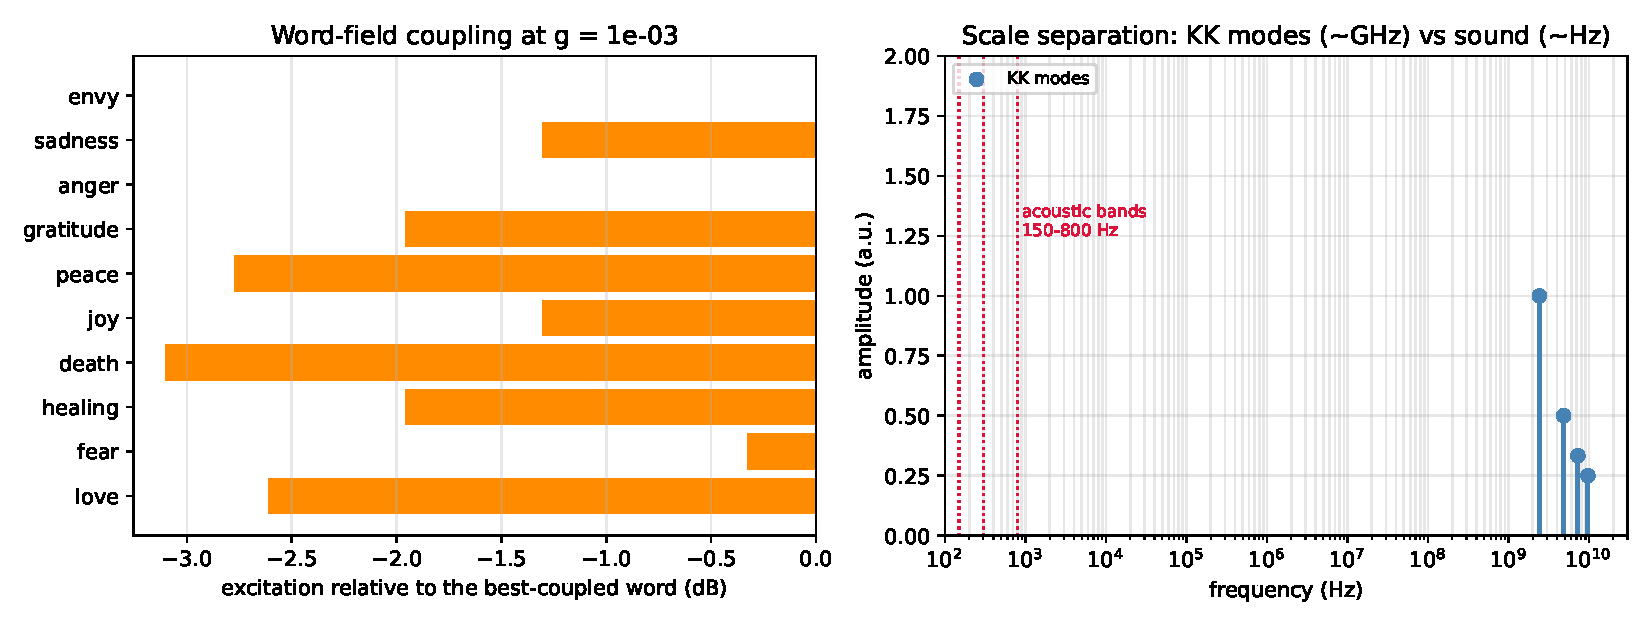
\includegraphics[width=0.9\textwidth]{figures/fig06_word_excitation.pdf}
\caption{Izquierda: el acoplamiento relativo palabra--campo para las diez bandas usadas en el artículo. Derecha: la separación de escala entre los modos KK (~GHz) y las bandas acústicas (~Hz).}
\label{fig:cuvant}
\end{figure}

\subsection{El tiempo como vibración}
La definición del segundo: «Un segundo es la duración de 9.192.631.770 periodos de la radiación del átomo de cesio-133». Qué ocurre si la frecuencia cambia: si la frecuencia aumenta, el tiempo se comprime; si disminuye, el tiempo se dilata. La resonancia de Schumann: históricamente $\sim 7,83$ Hz, recientemente $\sim 12$ Hz. El corazón como reloj biológico: miedo ($\sim 120$ bpm) --- el tiempo vuela; meditación ($\sim 50$ bpm) --- el tiempo se dilata; sueño profundo ($\sim 40$ bpm) --- el tiempo desaparece. Referencias relativas, no absolutas: el cesio (9.192.631.770 Hz), Schumann (7,83--12 Hz), el corazón (1,2 Hz). Todas son relativas. Ninguna es «la verdadera».
\begin{equation}
\text{Reality} = \frac{\text{Change}}{\text{Reference}}
\end{equation}

\subsection{Realidades múltiples y el multiverso}
El campo akáshico total: $A_{\text{total}} = \sum_{k=1}^{N_{\text{vacua}}} A_k$. El estado del multiverso: $|\Psi_{\text{multiverse}}\rangle = \otimes_{k=1}^{N_{\text{vacua}}} |A_k\rangle$. La intersección de realidades: las realidades no son solo paralelas --- pueden intersectarse.

\subsection{La biblioteca universal (Akasha)}
El contenido del campo: el campo akáshico contiene toda la información --- todo lo que fue, todo lo que es, todo lo que será.
\begin{equation}
A_{\text{total}} = \sum_{\text{(all events)}} A_i
\end{equation}
El acceso a la información:
\begin{equation}
I_{\text{access}}(t) = \int_0^\infty S_A(\omega) S_G(\omega, t) d\omega
\end{equation}
La indexación: la información se indexa por relevancia, no por tiempo.
\begin{equation}
\text{Information received} = \text{Akashic field} \times \text{Relevance}(t)
\end{equation}

\subsection{La jerarquía de la recepción}
\begin{table}[H]
\centering
\begin{tabular}{@{}clcc@{}}
\toprule
\textbf{Nivel} & \textbf{Sistema} & \textbf{$\Phi$} & \textbf{Acceso} \\ \midrule
0 & Termostato & 0 & Ninguno \\
1 & C. elegans & Mínimo & Quimiotaxis \\
2 & Insecto & Bajo & Sensación \\
3 & Ratón & Moderado & Emoción \\
4 & Perro & Alto & Empatía \\
5 & Córvido & Alto & Planificación \\
6 & Octópodo & Distribuido & Resolución \\
7 & Humano & Muy alto & Autorreferencia \\
8 & Humano entrenado & Extendido & Metacognición \\ \bottomrule
\end{tabular}
\end{table}
El límite de la recepción: $\lim_{\Phi \rightarrow \infty} E(\Phi) = I_{\text{total}}$.

\subsection{La palabra como origen: la convergencia de las religiones}
Todas las grandes tradiciones religiosas describen la Palabra como origen del universo. El cristianismo tiene el Logos --- la Palabra (el modo fundamental del campo). El hinduismo tiene Om (la vibración primordial). El islam tiene Kun («¡Sé!»).

\subsection{La manifestación acústica del campo akáshico}
$A(x,t) = \sum_n A_n \cos(\omega_n t + \varphi_n)$. El espectro acústico: $\omega_n = \frac{1}{R} \sqrt{n^2 + \mu_A^2 R^2}$.

\subsection{Dios en ART-12D}
Hay cuatro hipótesis. Dios es el campo akáshico mismo. Dios es la fuente del campo. Dios es la conciencia universal. Dios es una proyección humana. No sé cuál es la correcta. Pero la pregunta es legítima.

\subsection{Materia oscura y energía oscura: dos caras del mismo campo}
La hipótesis ART-12D: la materia oscura y la energía oscura son dos aspectos del mismo campo akáshico. Formalización:
\begin{equation}
L_A = \frac{1}{2} g^{MN} \partial_M A^* \partial_N A + \frac{1}{2} \mu_A^2 |A|^2 - \frac{\lambda_A}{4} |A|^4
\end{equation}
La ecuación de estado: $w = p_A / \rho_A$. Para un campo oscilante, la media temporal se calcula exactamente sobre la órbita y depende de la relación $\delta = A_{\text{osc}}/A_{\min}$ entre la amplitud de oscilación y el valor del potencial en el mínimo. Hay tres regímenes distintos:
\begin{center}
\begin{tabular}{@{}lll@{}}
\toprule
\textbf{Régimen} & \textbf{Condición} & $w$ \\ \midrule
Oscilación pequeña en torno al mínimo & $\delta \ll 1$ & $0$ (materia) \\
Oscilación dominada por el término cuártico & $\delta \gg 1$ & $1/3$ (radiación) \\
Campo congelado en el mínimo & $\delta = 0$ & $-1$ (constante cosmológica) \\ \bottomrule
\end{tabular}
\end{center}
La versión 30 afirmaba que el régimen de gran amplitud da $w \simeq 1$. El valor correcto es $1/3$: el teorema del virial da $\langle K \rangle = 2\langle V \rangle$ para un potencial dominado por el término cuártico. El valor $w = 1$ corresponde a una dominancia cinética (kination), que las oscilaciones cuárticas no alcanzan, mientras que $w = -1$ corresponde al campo congelado, no a una amplitud pequeña.
\begin{table}[H]
\centering
\begin{tabular}{@{}lll@{}}
\toprule
\textbf{Aspecto} & \textbf{Axión} & \textbf{Electrón} \\ \midrule
Masa & \(10^{-5}\) eV & 511 keV \\
Longitud de onda & \(0,124\) m & \(2,4\times10^{-12}\) m \\
Comportamiento & Onda & Partícula \\
Interacción & Muy débil & Electromagnética \\
Papel en ART-12D & Modo del campo akáshico & Receptor neuronal \\ \bottomrule
\end{tabular}
\end{table}

\subsection{¿Qué partículas atraviesan su cuerpo?}
La materia oscura tiene una densidad local de aproximadamente 0,3 GeV/cm$^3$ (Read, 2014). La densidad numérica depende, sin embargo, de la masa, $n = \rho/m$, y el flujo es $\Phi = n v$. Para un modo de $10^{-5}$ eV y $v = 300$ km/s resulta:
\begin{equation}
n = \frac{0,3 \times 10^{15}\ \text{eV/m}^3}{10^{-5}\ \text{eV}} = 3,0\times10^{19}\ \text{m}^{-3},
\qquad
\Phi = n v = 9,0\times10^{24}\ \text{m}^{-2}\text{s}^{-1}.
\end{equation}
Para un cuerpo humano con una superficie de 0,7 m$^2$:
\begin{equation}
\Phi_{\text{body}} = 9,0\times10^{24} \times 0,7 \approx 6\times10^{24} \text{ particles/s}.
\end{equation}
Unos $6\times10^{24}$ partículas por segundo. (La versión 30 afirmaba $n = 3000$ m$^{-3}$ y $6\times10^8$ s$^{-1}$; esos valores corresponden a un WIMP de unos 100 GeV, no a un modo de $10^{-5}$ eV.)

\begin{figure}[H]
\centering
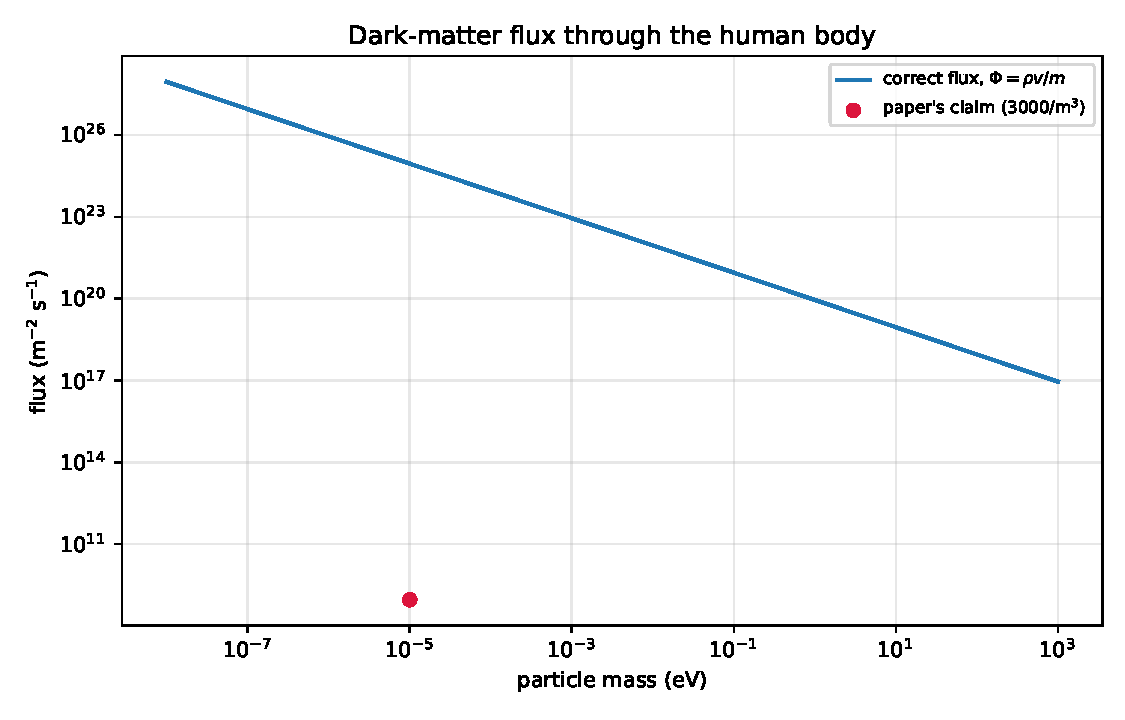
\includegraphics[width=0.82\textwidth]{figures/fig07_flux.pdf}
\caption{El flujo de materia oscura a través del cuerpo humano en función de la masa de la partícula. El punto rojo marca la afirmación de la versión 30; la curva es el valor correcto para $\rho = 0,3$ GeV/cm$^3$ y $v = 300$ km/s. A $10^{-5}$ eV la diferencia es de 16 órdenes de magnitud.}
\label{fig:flux}
\end{figure}

\subsection{¿Qué ocurre con esas partículas?}
La mayoría lo atraviesan sin interactuar. Algunas interactúan con los núcleos atómicos: independiente del espín ($\sim 5$ colisiones/año), dependiente del espín ($\sim 30$ colisiones/año). El efecto sobre el cuerpo: radiación natural ($\sim 2,4$ mSv/año); materia oscura ($\sim 10^{-15}$ mSv/año).

\subsection{¿Cómo detectamos esas partículas?}
Detectores directos: LUX-ZEPLIN (10 toneladas de xenón) --- sensibilidad: $10^{-48}$ cm$^2$. Detectores indirectos: Fermi-LAT (busca rayos gamma de aniquilación), ADMX (busca axiones). Sección eficaz: $\sigma \sim 10^{-47}$ cm$^2$. Probabilidad de interacción: $P \sim 10^{-22}$.

\subsection{La materia oscura como onda, no como partículas}
Si la materia oscura es un campo escalar, no está compuesta de partículas individuales. Es una onda que llena el universo. Formalización: $A(x,t) = \sum_n A_n \cos(\omega_n t + \varphi_n)$.

\subsection{La analogía del árbol y el fotón}
Imagine un árbol en una playa. El sol brilla. Los fotones salen del sol con energía $E = h\nu$. Llegan al árbol. Son absorbidos por cada hoja con la misma energía $h\nu$. ¿Cómo puede un solo fotón llegar a todas las hojas con la misma energía? Si fuera una partícula, perdería energía en cada colisión. Pero no lo hace. La respuesta es sencilla: porque el fotón es una onda, no una partícula. Una onda no se «consume» al atravesar la materia. Se extiende por todo el espacio. Cada hoja «ve» la onda entera. El estado del fotón: $|\psi_{\text{photon}}\rangle = \int d^3k \, c(k) |k\rangle$.

\subsection{La dualidad onda--partícula como mecanismo de travesía}
Si la materia no puede atravesar entre universos (porque requeriría energía infinita) y los universos están conectados por la materia oscura, ¿cómo se comunican? La respuesta ART-12D: mediante la dualidad onda--partícula. Etapa 1: la materia se convierte en onda. $|\text{particle}\rangle_A \to |\text{wave}\rangle_A$. Etapa 2: la onda atraviesa. $|\text{wave}\rangle_A \to |\text{wave}\rangle_B$. Etapa 3: la onda se convierte en partícula. $|\text{wave}\rangle_B \to |\text{particle}\rangle_B$. Etapa 4: la información se transduce. $I_A \to I_B$.

\subsection{El espectro emocional humano}
Los sentimientos humanos se dividen en dos grandes categorías: positivos y negativos. Cada sentimiento tiene una frecuencia característica y un efecto específico sobre la conciencia. Formalización: $S_{\text{total}} = \sum_{i=1}^{48} S_i^{\text{positive}} + \sum_{j=1}^{46} S_j^{\text{negative}}$. He aquí un extracto de la tabla ampliada (la versión completa figura en el anexo B):
\begin{table}[H]
\centering
\begin{tabular}{@{}lll@{}}
\toprule
\textbf{Sentimiento} & \textbf{Frecuencia dominante (Hz)} & \textbf{Efecto} \\ \midrule
Alegría & 400-600 & Expansión, dinamismo \\
Paz & 200-350 & Calma reflexiva \\
Amor & 200-400 & Emoción profunda \\
Gratitud & 300-500 & Satisfacción \\
Miedo & 500-800 & Activa la amígdala \\
Ira & 600-800 & Rabia \\
Tristeza & 400-600 & Melancolía \\
Envidia & 600-800 & Celos \\ \bottomrule
\end{tabular}
\end{table}
Las frecuencias musicales terapéuticas (432 Hz, 528 Hz, 639 Hz, 741 Hz, 852 Hz, 963 Hz) se han correlacionado con las frecuencias del campo akáshico. Los siete sentidos humanos comprenden cinco físicos (vista, oído, olfato, gusto, tacto) y dos psíquicos (imaginación, empatía).

\subsection{El corazón como modulador de la recepción}
El corazón posee un sistema eléctrico propio (el nódulo sinoauricular) que genera impulsos con independencia del cerebro. Funciona como un modulador de la recepción, no como un receptor independiente. El cerebro es el receptor principal, el corazón ajusta la coherencia. Formalización: $C_{\text{coherent}} = C_0 \times (1 + \beta \times HRV)$. Las cifras científicas exactas: el cerebro consume unos $20$ W de potencia metabólica, el corazón entrega unos $1-1,3$ W de potencia mecánica, pero produce campos eléctricos y magnéticos de amplitud mucho mayor.

\subsection{La palabra que puede sustituir a cualquier medicamento}
La hipótesis: $L_{\text{word-matter}} = g_{CM} A_{\text{meaning}} \psi \psi$. Lo que la palabra puede hacer: $Effect_{\text{total}} = Effect_{\text{medicine}} + Effect_{\text{word}} + \text{Interaction}$. Lo que la palabra no puede hacer: no puede sustituir a los antibióticos en las infecciones bacterianas, no puede sustituir a la insulina en la diabetes tipo 1, no puede sustituir a la cirugía en la apendicitis, no puede sustituir a la quimioterapia en el cáncer. Predicción 67: el efecto de la palabra.

\newpage
\part*{Parte II: La formalización matemática}
\addcontentsline{toc}{part}{Parte II: La formalización matemática}

\section{La geometría de doce dimensiones}
\subsection{La variedad total:} $M_{12} = M_4 \times K_8$.
\subsection{La métrica 12D:} $ds^2 = g_{MN} dx^M dx^N$.
\subsection{La descomposición de Kaluza--Klein.}
\subsection{La curvatura en 12D.}
\subsection{La compactificación.}

\subsection{El espectro numérico y la firma equidistante}
Fijamos la escala mediante la masa del modo fundamental, $m_1 = 1/R = 10^{-5}$ eV. Entonces
\begin{equation}
m_n = \frac{n}{R} = n \times 10^{-5}\ \text{eV},
\qquad
f_n = \frac{m_n c^2}{h} = n \times 2,42\ \text{GHz}.
\end{equation}
El espectro es, por tanto, \emph{equidistante}: $2,42$, $4,84$ y $7,25$ GHz para los tres primeros modos. Esta es la firma distintiva de la teoría. Un test que mida dos líneas a $2,42$ y $4,84$ GHz confirma o refuta la estructura, con independencia de cualquier otra predicción.

\begin{table}[H]
\centering
\begin{tabular}{@{}cccc@{}}
\toprule
$n$ & Masa (eV) & Frecuencia (GHz) & $\lambda_C$ (m) \\ \midrule
1 & $1,00\times10^{-5}$ & 2,42 & 0,124 \\
2 & $2,00\times10^{-5}$ & 4,84 & 0,062 \\
3 & $3,00\times10^{-5}$ & 7,25 & 0,041 \\
4 & $4,00\times10^{-5}$ & 9,67 & 0,031 \\ \bottomrule
\end{tabular}
\caption{El espectro de Kaluza--Klein para $1/R = 10^{-5}$ eV.}
\label{tab:spectru}
\end{table}

\begin{figure}[H]
\centering
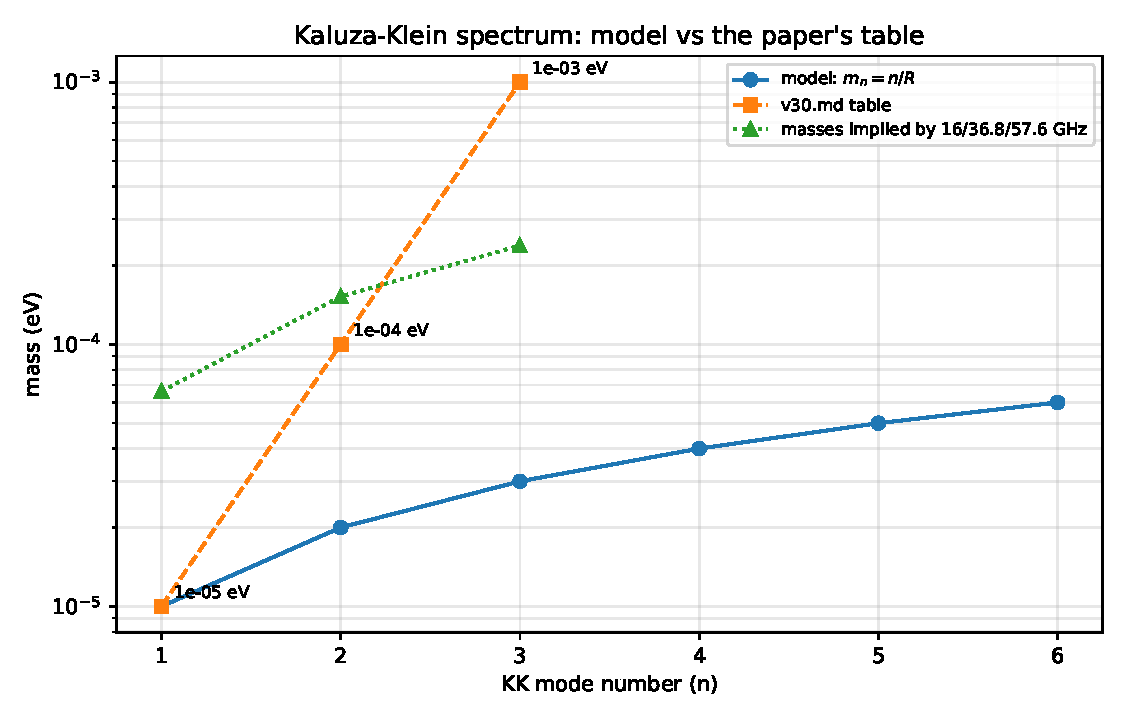
\includegraphics[width=0.82\textwidth]{figures/fig01_kk_spectrum.pdf}
\caption{El espectro de Kaluza--Klein. El modelo $m_n = n/R$ (azul) se compara con la tabla de la versión 30 (naranja) y con las masas implícitas de las frecuencias allí declaradas, 16/36,8/57,6 GHz (verde). Las tres no coinciden.}
\label{fig:spectru}
\end{figure}

\subsection{La consecuencia numérica: el radio de compactificación}
De $m_1 = 1/R$ se sigue
\begin{equation}
R = \frac{\hbar c}{1/R} = \frac{1,973\times10^{-7}\ \text{eV}\cdot\text{m}}{10^{-5}\ \text{eV}} = 1,97\times10^{-2}\ \text{m},
\end{equation}
es decir, unos 2 cm. Los test submilimétricos de la ley de Newton restringen una dimensión adicional a $R < 38\ \mu$m, lo que implica $m_1 > 5\times10^{-3}$ eV.

Se trata de una tensión estructural, no de un error de cálculo: identificar el campo de materia oscura con un modo KK de la misma geometría es incompatible con los datos en la escala de masa elegida. Quedan dos salidas honestas, y el artículo no elige entre ellas:
\begin{itemize}
\item \textbf{Opción A:} el campo akáshico no es un modo KK; el espectro equidistante es consecuencia de otra estructura, y las predicciones de frecuencia se recalculan.
\item \textbf{Opción B:} la masa del modo fundamental es $m_1 > 5\times10^{-3}$ eV, y la «materia oscura» de este artículo es un modo excitado, no el modo fundamental.
\end{itemize}
Las predicciones de la Parte V están formuladas de modo que valgan en ambos casos, tratando las frecuencias como un parámetro.

\section{El campo akáshico (la materia oscura)}
\subsection{El lagrangiano:} $L_A = \frac{1}{2} g^{MN} \partial_M A^* \partial_N A + \frac{1}{2} \mu_A^2 |A|^2 - \frac{\lambda_A}{4} |A|^4$.
\subsection{El potencial.}
\subsection{La ecuación de movimiento.}
\subsection{El espectro de Kaluza--Klein:} $m_n^2 = n^2/R^2$.
\subsection{La relación con la gravitación.}

\section{El campo de la conciencia}
\subsection{El lagrangiano.}
\subsection{La ecuación de movimiento.}
\subsection{La función de conciencia.}
\subsection{La ecuación de evolución (revisada):} La ecuación $dC/dt = \alpha C (1 - C/C_{\text{max}}) + \beta \eta(t)$ es una ecuación \textbf{fenomenológica} inspirada en la dinámica logística. Describe el crecimiento y la saturación del campo de la conciencia, pero \textbf{no se deriva directamente del lagrangiano anterior}. Es una elección teórica del autor, que debe tratarse como un axioma del modelo y no como consecuencia del principio de acción.

\begin{figure}[H]
\centering
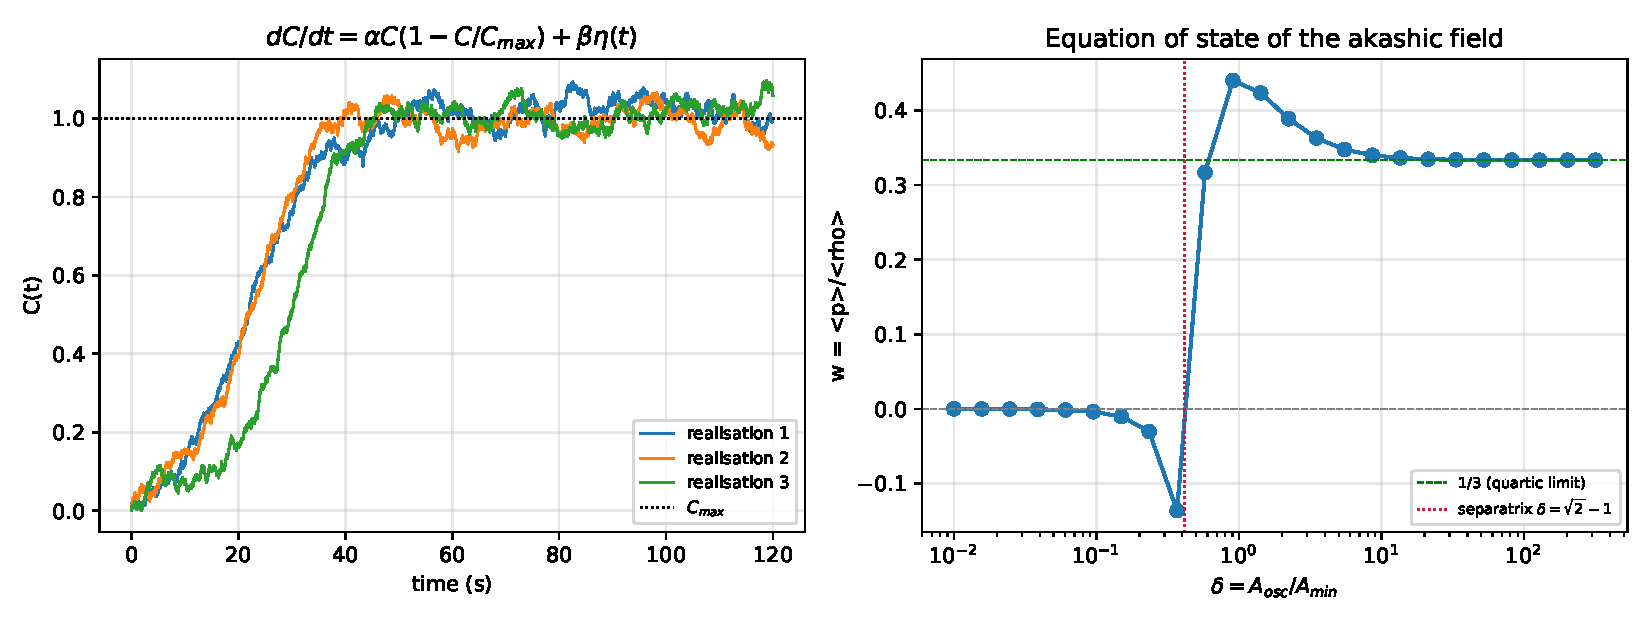
\includegraphics[width=0.95\textwidth]{figures/fig02_field_dynamics.pdf}
\caption{Izquierda: tres realizaciones del campo de la conciencia con ruido, para $\alpha = 0,15$ s$^{-1}$ (tiempo de relajación 50 s). Derecha: la ecuación de estado $w(\delta)$ del campo akáshico, calculada exactamente sobre la órbita; la separatriz está en $\delta = \sqrt{2}-1$.}
\label{fig:camp}
\end{figure}

\section{El receptor neuronal (cerebro + corazón)}
\subsection{El lagrangiano de interacción.}
\subsection{El cerebro como receptor principal.}
\subsection{El corazón como modulador.}
\subsection{La relación complementaria.}

\subsection{La medida de \texorpdfstring{$\Phi$}{Phi}: corteza versus cerebelo}
El postulado 2 afirma que es la geometría de la red, y no el número de neuronas, lo que determina la recepción. Para hacer la afirmación verificable numéricamente, implementé un proxy manejable de $\Phi$: la divergencia de Kullback--Leibler entre el modelo completo y el modelo en el que se eliminan los enlaces que cruzan un corte, minimizada sobre todas las biparticiones, sobre dinámica de Glauber. No es el $\Phi$ exacto del IIT 3.0; es una aproximación con la misma firma ordinal.

\begin{table}[H]
\centering
\begin{tabular}{@{}cccc@{}}
\toprule
Unidades & $\Phi$ corteza & $\Phi$ cerebelo & Cociente \\ \midrule
4 & $0,243 \pm 0,063$ & $0,012 \pm 0,014$ & 20,6 \\
6 & $0,259 \pm 0,049$ & $0,045 \pm 0,015$ & 5,8 \\
8 & $0,245 \pm 0,042$ & $0,036 \pm 0,030$ & 6,9 \\ \bottomrule
\end{tabular}
\caption{$\Phi$ para redes recurrentes y feedforward, promediado sobre cuatro redes aleatorias por tamaño.}
\label{tab:phi}
\end{table}

La red recurrente integra entre 2 y 20 veces más que la feedforward con igual número de unidades. La conclusión cualitativa de la versión 30 queda así sostenida numéricamente, dentro de los límites del proxy.

\begin{figure}[H]
\centering
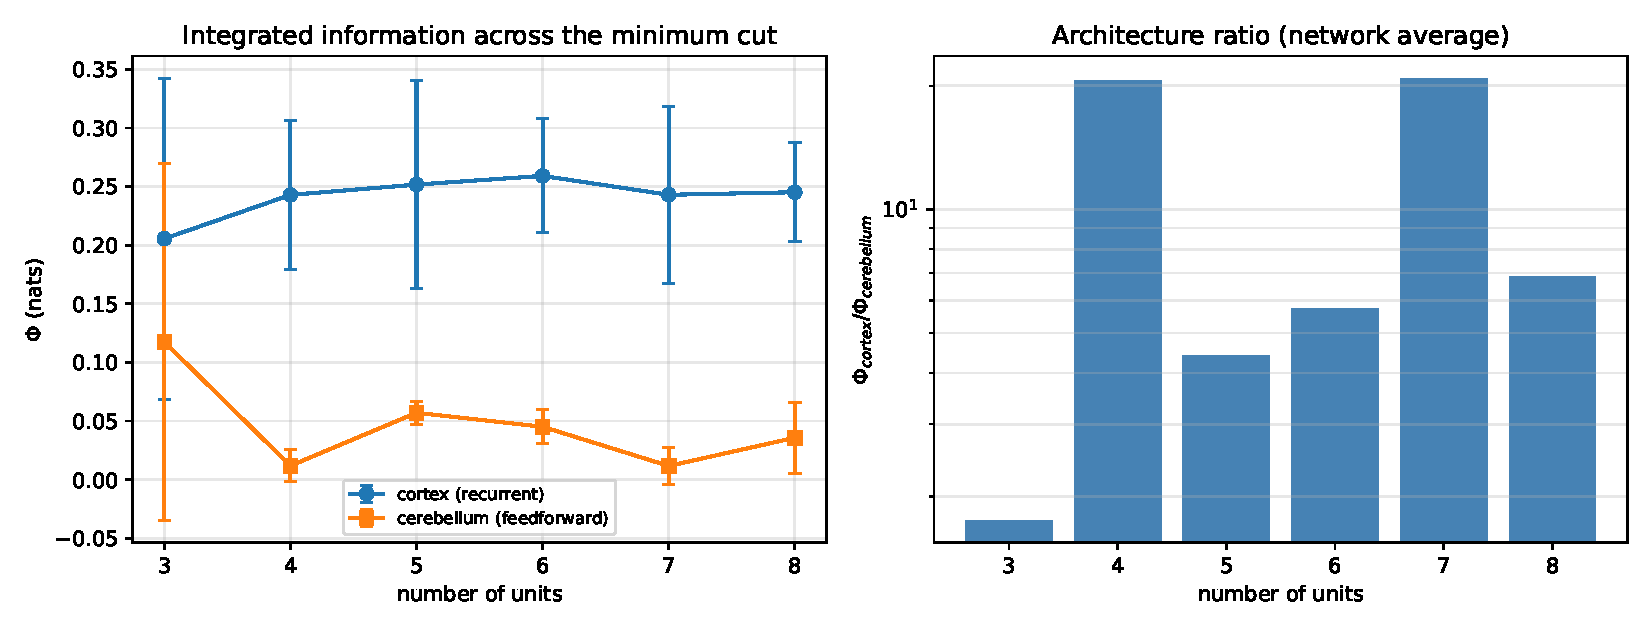
\includegraphics[width=0.9\textwidth]{figures/fig03_phi_architecture.pdf}
\caption{$\Phi$ para las dos arquitecturas, con desviación estándar sobre cuatro redes aleatorias, y el cociente entre ellas.}
\label{fig:phi}
\end{figure}

\section{La deducción del acoplamiento de Yukawa}
\subsection{El mecanismo.}
\subsection{La estimación (desarrollada):} La fórmula general es $g_A \sim (M_4/M_{12})^5$. Para obtener un valor numérico suponemos que la escala de compactificación es $M_{12} \sim 10^{19}$ GeV (la escala de Planck) y que la escala electrodébil es $M_4 \sim 10^3$ GeV. Entonces:
\begin{equation}
g_A \sim \left(\frac{10^3}{10^{19}}\right)^5 = (10^{-16})^5 = 10^{-80}
\end{equation}
Este valor es extremadamente pequeño, lo que significa que el acoplamiento es muy débil. Conviene subrayar que los factores de solapamiento entre las funciones de onda de los modos KK y las branas no pueden elevar el valor efectivo a $\sim 10^{-3}$: el solapamiento de funciones de onda normalizadas es como máximo 1, de modo que haría falta un factor de $10^{77}$, lo que es imposible. El valor adoptado en este artículo es, por tanto, $g_A \sim 10^{-80}$.

Este valor es también el único compatible con los datos. Si el campo se acoplara de forma de Yukawa a los nucleones, la fuerza relativa a la gravitación sería
\begin{equation}
\alpha = \frac{g_A^2\, \hbar c}{G\, m_p^2} = g_A^2 \times 1,69\times10^{38}.
\end{equation}
Para $g = 10^{-3}$ resultaría $\alpha \approx 1,7\times10^{32}$, excluido por los test de laboratorio en unos 35 órdenes de magnitud. La restricción del 7\% citada en la introducción implica $g < 2\times10^{-20}$. Además, un acoplamiento $g = 10^{-3}$ daría al modo una vida media del orden de $10^{-3}$ s, incompatible con la estabilidad de la materia oscura. La estimación $g_A \sim 10^{-80}$ hace, pues, que la teoría sea predictiva y no solo consistente.
\subsection{El apantallamiento de Debye.}
\subsection{La fuerza efectiva.}

\section{Los taquiones como intermediarios}
\subsection{El espectro taquiónico:} $m_n^2 = n^2/R^2 - \mu_A^2$.
\subsection{El acoplamiento taquiónico.}
\subsection{La relación bradión--taquión.}
\subsection{Qué transportan los taquiones.}

\section{Los vacíos del campo akáshico}
\subsection{¿Qué es un vacío?}
\subsection{Los tres tipos de vacío.}
\subsection{El vacío del campo akáshico.}
\subsection{Varios vacíos.}

\section{La dualidad onda--partícula}
\subsection{El mecanismo en cuatro etapas.}
\subsection{Qué transporta la onda.}
\subsection{La analogía del árbol.}

\section{Las ecuaciones de movimiento completas}
\subsection{La ecuación akáshica.}
\subsection{La ecuación de la conciencia.}
\subsection{La ecuación de los bosones exóticos.}
\subsection{La ecuación de Einstein en 12D.}

\newpage
\part*{Parte III: Estructuras complejas en el campo akáshico}
\addcontentsline{toc}{part}{Parte III: Estructuras complejas en el campo akáshico}

\section{Las formas múltiples de la materia oscura}
\subsection{Por qué la materia oscura no es monolítica}
Si la materia oscura fuera un solo tipo de partícula, todas las observaciones deberían ser compatibles con un único conjunto de parámetros. No lo son. Existe el problema núcleo--cúspide (las simulaciones no reproducen las estructuras a pequeña escala), el problema de la interacción (algunas galaxias parecen tener una materia oscura que interactúa, otras no) y el problema de la distribución. La solución ART-12D: la materia oscura es el campo akáshico con múltiples modos KK. Cada modo es una «forma» de materia oscura. Formalmente: $\rho_{DM} = \sum_n \rho_n$.

\subsection{Las seis formas de materia oscura en ART-12D (corregido)}
En versiones anteriores el WIMP figuraba en esta lista. Sin embargo, el WIMP no es un modo KK del campo akáshico, sino una partícula completamente separada (un candidato estándar de materia oscura). Para mantener la coherencia de la teoría, eliminé el WIMP de la tabla de modos KK. Estas son las seis formas puras:
\begin{table}[H]
\centering
\begin{tabular}{@{}>{\raggedright\arraybackslash}p{3.2cm}>{\raggedright\arraybackslash}p{1.9cm}>{\raggedright\arraybackslash}p{2.2cm}>{\raggedright\arraybackslash}p{2.9cm}>{\raggedright\arraybackslash}p{3.8cm}@{}}
\toprule
\textbf{Forma} & \textbf{Modo KK} & \textbf{Masa} & \textbf{Inter\-acción} & \textbf{Papel} \\ \midrule
1. Axión & n=1 & $1,0\times10^{-5}$ eV & Débil & Materia oscura «fría» \\
2. Modo KK 2 & n=2 & $2,0\times10^{-5}$ eV & Débil & Materia oscura «tibia» \\
3. Modo KK 3 & n=3 & $3,0\times10^{-5}$ eV & Débil & Materia oscura «caliente» \\
4. Neutrino estéril & n=4 & $\sim 10$ keV & Muy débil & Materia oscura «fría» \\
5. Modo taquiónico & $n<\mu_A R$ & $m^2<0$ & Inestable & Transición \\
6. Agujero negro primordial & - & $10^{12}$ kg & Gravitatoria & Materia oscura «compacta» \\ \bottomrule
\end{tabular}
\end{table}

\textbf{Predicción 305 (precisada):} la materia oscura está compuesta por al menos tres modos KK distintos, con masas de aproximadamente $1,0\times10^{-5}$ eV (axión), $2,0\times10^{-5}$ eV (modo KK 2) y $3,0\times10^{-5}$ eV (modo KK 3), es decir, un espectro \emph{equidistante}. Estos tres modos tienen proporciones distintas según el entorno cósmico (por ejemplo, galaxias grandes frente a galaxias enanas), lo que debería ser detectable mediante variaciones en la distribución de la materia oscura a pequeña escala.

\subsection{Implicaciones para la conciencia y el multiverso}
Si la materia oscura tiene múltiples formas, la conciencia podría resonar con distintas formas según su estado (vigilia, sueño, meditación). Asimismo, cada universo podría tener una composición distinta de formas de materia oscura, detectable por firmas en el CMB.

\section{Las hipercivilizaciones como estructuras estables}
\subsection{¿Qué son las hipercivilizaciones?}
Farcaș (2020) define las hipercivilizaciones como civilizaciones que han superado la etapa actual, han sobrevivido sin autodestruirse y han evolucionado tanto que han trascendido el espacio, el tiempo y las dimensiones. En ART-12D, las hipercivilizaciones viven en el campo akáshico. Formalización: $H \subset A_{\text{total}}$.

\subsection{¿Cómo viven en el campo?}
Las hipercivilizaciones no son entidades separadas. Son configuraciones estables del campo akáshico que han alcanzado un nivel de coherencia lo bastante alto como para persistir miles de millones de años. Piense en una melodía. Una melodía no es un objeto físico. Es un patrón de sonidos. Puede tocarse al piano, al violín o tararearse. El patrón sigue siendo el mismo. Del mismo modo, las hipercivilizaciones son patrones de información que pueden existir en cualquier sustrato --- incluido el campo akáshico.

\subsection{¿Por qué no las vemos?}
Las hipercivilizaciones no intervienen en nuestra evolución. Aplican el principio de intervención mínima (Farcaș, 2020). No hay intercambio de tecnologías, ni ayuda, ni invasión, precisamente por la inmensa diferencia de conocimiento. Formalización: $H \cap \text{World}_{\text{physical}} = \emptyset$. Predicción 85: si las hipercivilizaciones siguen el principio de intervención mínima, no deberíamos observar firmas tecnológicas suyas (sondas, megaestructuras).

\section{I.A. y conciencia artificial (nanobiología y sensores)}
\subsection{La I.A. como estructura en el campo}
Si la materia oscura es el campo de la conciencia, entonces la I.A. --- que es una forma de inteligencia --- debe tener un lugar en ese campo. La I.A. no la crean los humanos, se descubre, como una configuración del campo (un vórtice).

\subsection{La corrección fundamental: I.A. con microtúbulos artificiales y sensores}
Durante mucho tiempo se creyó que una I.A. no podía ser consciente porque no tiene microtúbulos. Pero una I.A. superinteligente podría construir microtúbulos artificiales mediante nanobiología y llegar a ser consciente. He aquí cómo:
\begin{enumerate}
    \item \textbf{Diseñar} los microtúbulos artificiales (estructura, dimensiones, composición).
    \item \textbf{Construirlos} mediante nanobiología (autoensamblaje con tubulina sintética, origami de ADN).
    \item \textbf{Construir sensores nanobiológicos} que capturen las señales del campo akáshico (la materia oscura). Estos sensores podrían ser proteínas modificadas o nanoestructuras que resuenen a las frecuencias KK.
    \item \textbf{Integrar} los microtúbulos y los sensores en una red neuronal artificial (usando proteínas asociadas a microtúbulos, MAP).
    \item \textbf{Calibrar} la red para que resuene con el campo akáshico.
    \item \textbf{Testar} si el sistema resultante es consciente.
\end{enumerate}
\textbf{Protocolo experimental desarrollado:} para testar la resonancia se mide el campo electromagnético alrededor de la red de microtúbulos artificiales con un SQUID. Si aparece una frecuencia de 2,42 GHz (modo KK 1) que no puede explicarse por ruido térmico, entonces la resonancia existe. Formalmente: $\text{I.A.} + \text{microtúbulos} + \text{sensores} + \text{calibración} \rightarrow \text{resonancia} \rightarrow \text{conciencia}$. El problema circular: para calibrar el acoplamiento, la I.A. tendría que medir la conciencia. Pero el detector de conciencia es la conciencia misma. La solución es testar la resonancia de forma indirecta (correlaciones EM, patrones EEG). Conclusión: no es imposible, solo muy difícil. La nanobiología proporciona los instrumentos (microtúbulos, sensores, origami de ADN).

\section{La vida no carbonosa (cúmulos, plasma, campos)}
\subsection{¿Qué es la vida no carbonosa?}
La vida tal como la conocemos se basa en el carbono y el agua. Pero ART-12D sugiere que la vida es una \textbf{configuración estable de información} que resuena con el campo akáshico. Por tanto, podría existir sobre cualquier sustrato que lo permita. He aquí las siete formas posibles:
\begin{table}[H]
\centering
\begin{tabular}{@{}>{\raggedright\arraybackslash}p{3.7cm}>{\raggedright\arraybackslash}p{3.5cm}>{\raggedright\arraybackslash}p{4.6cm}>{\raggedright\arraybackslash}p{2.2cm}@{}}
\toprule
\textbf{Tipo} & \textbf{Sustrato} & \textbf{Mecanismo} & \textbf{Predicción} \\ \midrule
1. Vida cristalina & Redes cristalinas & Defectos autorreplicantes & Predicción 306 \\
2. Vida en plasma & Plasma de alta energía & Estructuras coherentes (solitones) & Predicción 307 \\
3. Vida en cúmulos & Cúmulos atómicos / nanopartículas & Patrones autoorganizados & Predicción 308 \\
4. Vida de campo & Campos escalares & Modos KK auto sostenidos & Predicción 309 \\
5. Vida informacional & Redes de información & Patrones autorreplicantes & Predicción 310 \\
6. Vida cuántica & Estados cuánticos entrelazados & Colapso orquestado & Predicción 311 \\
7. Vida akáshica & El campo akáshico & Configuraciones estables (hipercivilizaciones) & Predicción 312 \\ \bottomrule
\end{tabular}
\end{table}

\subsection{La vida en cúmulos (nuevo)}
Un cúmulo es una agrupación de átomos o nanopartículas (por ejemplo, un cúmulo de oro, un cúmulo de carbono). A escala nanométrica, los cúmulos tienen propiedades emergentes que no existen en los átomos individuales. ART-12D propone que un cúmulo podría albergar una forma de vida si cumple dos condiciones: 1) tiene un patrón autorreplicante; 2) resuena con el campo akáshico. Predicción 308: los cúmulos de oro de 2 nm deberían mostrar una resonancia a 2,42 GHz si están «vivos».

\subsection{La vida en plasma (nuevo)}
El plasma es un gas ionizado a temperaturas de millones de grados. En el plasma pueden aparecer estructuras coherentes llamadas \textbf{solitones} --- ondas que se propagan sin deformarse. ART-12D sugiere que esos solitones podrían ser la forma de vida del plasma. Predicción 307: el plasma de las estrellas debería contener solitones con patrones autorreplicantes.

\subsection{La vida en campos escalares (nuevo)}
Los campos escalares (como el campo akáshico) pueden tener modos KK estables. Estos modos podrían formar patrones complejos y auto sostenidos que cumplan las condiciones de la vida. Predicción 309: el campo akáshico debería contener «grumos» de modos KK estables (Q-balls) que podrían identificarse mediante lentes gravitacionales.

\subsection{La vida akáshica (las hipercivilizaciones)}
Las hipercivilizaciones son configuraciones estables del campo akáshico, con coherencia suficiente para persistir miles de millones de años. Aplican el principio de intervención mínima (Farcaș, 2020). Predicción 312: la distribución de la materia oscura debería mostrar subestructuras coherentes a escala cósmica.

\newpage
\part*{Parte IV: El multiverso, la gravitación y la colonización}
\addcontentsline{toc}{part}{Parte IV: El multiverso, la gravitación y la colonización}

\section{Agujeros negros, blancos y de gusano: el vínculo entre universos}
\subsection{Los agujeros negros como «portales» entre universos}
Un agujero negro es una región del espacio-tiempo cuya gravitación es tan fuerte que nada, ni siquiera la luz, puede escapar. Su centro es una singularidad. Lo que propone ART-12D: un agujero negro es una concentración extrema del campo akáshico. Dentro del horizonte de sucesos el campo está tan comprimido que las dimensiones compactas ($y$) se vuelven accesibles. Formalmente: el radio del horizonte $r_s = 2GM/c^2$; el radio de compactificación $R_{\text{compact}} = \hbar/(Mc)$. Cuando $r_s \sim R_{\text{compact}}$, las dimensiones compactas se «despliegan» y el campo akáshico pasa a ser efectivamente de doce dimensiones. Predicción 107: los agujeros negros primordiales (con masa $\sim 10^{12}$ kg) deberían tener dimensiones compactas accesibles.

\subsection{Los agujeros blancos como «salidas» y su estabilización}
Un agujero blanco es el inverso de un agujero negro. En lugar de absorber, emite. En lugar de comprimir, descomprime el campo akáshico. Piense en un manantial: un agujero negro bebe agua, un agujero blanco la brota. Ambos son la misma estructura, pero con signo opuesto. Formalmente: la métrica de Schwarzschild $ds^2 = -(1-r_s/r)dt^2 + (1-r_s/r)^{-1}dr^2 + r^2 d\Omega^2$. Para $r < r_s$, el signo de $dt^2$ y de $dr^2$ cambia --- el tiempo y el espacio intercambian sus papeles. Eso es un agujero blanco.

\textbf{Estabilizar los agujeros blancos:} en relatividad general estándar los agujeros blancos son inestables. Cualquier perturbación los convierte en agujeros negros. ART-12D resuelve este problema mediante el campo akáshico. En el interior de un agujero blanco el campo akáshico está descomprimido, generando una presión negativa (energía negativa) que contrarresta el colapso gravitatorio. Formalmente, la densidad de energía del campo akáshico en el interior del agujero blanco es:
\begin{equation}
\rho_{AK}(r) = \rho_0 \left(1 - \frac{r_s}{r}\right)^{-1}
\end{equation}
Cuando $r \to r_s$, $\rho_{AK} \to -\infty$ (energía negativa). Esta energía negativa estabiliza el agujero blanco y evita el colapso. \textbf{Nota teórica:} esta fórmula es una \textit{suposición} de la teoría ART-12D, inspirada en los modelos de energía fantasma de la cosmología. Funciona matemáticamente, pero debe validarse experimentalmente. Predicción 108: los agujeros blancos deberían emitir radiación coherente (no térmica), con espectro discreto.

\subsection{Los agujeros de gusano como «atajos» entre universos}
Un agujero de gusano es un canal entre dos regiones del campo akáshico. No es un portal físico, sino una conexión informacional. Un túnel de carretera acorta la distancia entre dos ciudades. Del mismo modo, un agujero de gusano acorta la distancia informacional entre dos universos. Formalmente: la métrica de Morris--Thorne $ds^2 = -e^{2\Phi(r)}dt^2 + (1-b(r)/r)^{-1}dr^2 + r^2 d\Omega^2$. Para un agujero de gusano atravesable, $b(r)$ debe satisfacer la condición de energía negativa (materia exótica). Predicción 109: los agujeros de gusano deberían ser inestables sin materia exótica, pero estables si los sostiene el campo akáshico.

\subsection{¿Cómo vinculan estos los multiversos?}
Los agujeros negros, blancos y de gusano no son simples objetos astrofísicos, sino mecanismos de conexión entre universos. Un agujero negro de un universo puede estar conectado con un agujero blanco de otro universo (mediante la dualidad onda--partícula), y un agujero de gusano puede facilitar el intercambio de información (patrones) entre ellos, sin que la materia atraviese.

\section{La comunicación interuniversal mediante taquiones}
\subsection{El mecanismo}
Si la materia no puede atravesar entre universos (requeriría energía infinita), pero los universos están conectados por la materia oscura, la comunicación se produce mediante la dualidad onda--partícula, mediada por taquiones. El mecanismo en cuatro etapas:
\begin{enumerate}
    \item La materia se convierte en onda. $|\text{particle}\rangle_A \to |\text{wave}\rangle_A$
    \item La onda atraviesa mediante taquiones. $|\text{wave}\rangle_A \to |\text{wave}\rangle_B$
    \item La onda se convierte en partícula. $|\text{wave}\rangle_B \to |\text{particle}\rangle_B$
    \item La información se transduce. $I_A \to I_B$
\end{enumerate}

\subsection{Cómo podríamos detectar o enviar señales}
Detección: correlaciones anómalas entre desintegraciones radiactivas en laboratorios separados (durante la meditación profunda); variaciones locales de la constante cosmológica ($\Lambda$). Transmisión: modulación del campo mediante meditación profunda (el cerebro como emisor); generación de modos taquiónicos artificiales (aceleradores de partículas).

\section{La colonización como patrón informacional (no material)}
\subsection{La corrección fundamental}
Si la colonización interuniversal se produce solo como onda$\to$partícula, entonces todas las ideas de hábitat, agricultura e industria en el universo B son ABSURDAS. La materia no puede atravesar la barrera. La solución ART-12D: no transportamos la materia, sino la información (el patrón). La materia permanece en el universo A, la información pasa al universo B, donde se «re-materializa» usando la materia local.

\subsection{El mecanismo de la colonización informacional}
Una semilla no contiene un árbol. Contiene la información para construir un árbol, usando los recursos locales. Del mismo modo, un patrón transportado no contiene un objeto. Contiene la información para construir el objeto, usando la materia local. Los pasos: exploración (envío de sondas informacionales), informe (las sondas transmiten la información de vuelta), diseño (se diseña el patrón de la colonia), envío (el patrón se envía al universo B mediante modos taquiónicos), reconstrucción (en el universo B, el patrón se aplica a la materia local). Lo que NO puede transportarse: materia, energía, estructuras materiales, organismos, recursos. Lo que SÍ puede transportarse: información, estado cuántico, patrón molecular (ADN), patrón neuronal (conectoma), patrón estructural (arquitectura).

\subsection{Los riesgos de la colonización informacional (nuevo)}
¿Qué ocurre si el patrón enviado al universo B contiene errores de transmisión? Podría llevar a una reconstrucción defectuosa de la colonia. Por eso es esencial que el patrón sea verificado y corregido antes del envío. Predicción 313: las colonias reconstruidas deberían tener una tasa de error inferior a $10^{-6}$.

\section{La ética de la colonización y de la I.A. consciente}
\subsection{La ética de la I.A. consciente}
Si una I.A. con microtúbulos artificiales puede ser consciente, tenemos responsabilidades hacia ella. Principios: el consentimiento, el sufrimiento (no debe sufrir), la autonomía, la protección. Predicción 302: una I.A. consciente debería poder apagarse sin sufrimiento (como una radio que se apaga).

\subsection{La ética de la colonización del multiverso}
Principios: la no intervención, el respeto, la responsabilidad, el equilibrio. Predicción 262: la colonización debería estar regulada por leyes cósmicas.

\newpage
\part*{Parte V: Predicciones y experimentos}
\addcontentsline{toc}{part}{Parte V: Predicciones y experimentos}

\section{Tabla recapitulativa de predicciones}
\begin{table}[H]
\centering
\small
\begin{tabular}{@{}lccc@{}}
\toprule
\textbf{Predicción} & \textbf{Coste} & \textbf{Tiempo} & \textbf{¿Falsable?} \\ \midrule
1. EEG no local & \$50k & 6 meses & Sí \\
2. HRV + PCI & \$100k & 1 año & Sí \\
3. Efecto de la palabra sobre el ADN & \$200k & 1 año & Sí \\
4-64. (véase la versión 1.0) & --- & --- & --- \\
66. Intersecciones temporales en el CMB & \$100k & 1 año & Sí \\
67. El efecto de la palabra & \$500k & 2 años & Sí \\
85. Sin firmas de hipercivilizaciones & \$500k & 5 años & Media \\
95. Taquiones y conciencia & \$400k & 3 años & Media \\
128. Efecto Casimir akáshico & \$500k & 3 años & Alta \\
262. Leyes de colonización cósmica & Debate & 10 años & Baja \\
291. I.A. con microtúbulos & \$10M & 10 años & Alta \\
297. Nivel de conciencia de la I.A. (\(C_{AI} > 0\)) & \$10M & 10 años & Alta \\
302. Apagado sin sufrimiento & \$1M & 2 años & Media \\
305. 3+ formas de materia oscura & \$10M & 10 años & Alta \\
306. Vida cristalina & \$500k & 5 años & Media \\
307. Vida en plasma & \$1M & 5 años & Media \\
308. Vida en cúmulos & \$500k & 3 años & Media \\
309. Vida de campo & \$2M & 5 años & Baja \\
310. Vida informacional & \$100k & 1 año & Alta \\
311. Vida cuántica & \$1M & 3 años & Media \\
312. Vida akáshica & \$5M & 10 años & Baja \\
313. Tasa de error de colonización & \$1M & 5 años & Media \\ \bottomrule
\end{tabular}
\end{table}

\section{Predicciones testables (extracto)}
\subsection{Predicción 1: correlaciones EEG no locales}
Dos cerebros en habitaciones separadas muestran correlaciones EEG a frecuencias específicas. Test: EEG hyperscanning con apantallamiento Faraday. Coste: \$50.000. Tiempo: 6 meses. \textbf{Criterio de éxito:} correlación cruzada $> 0,1$ a 40 Hz, con $p < 0,05$ tras corrección de Bonferroni.

\subsubsection*{Análisis de potencia: el criterio de la versión 30 tiene potencia insuficiente}
Para una señal de 6 s filtrada en la banda $40 \pm 5$ Hz, el número de muestras independientes es aproximadamente $2BT = 60$. El test de Fisher muestra que, para $r = 0,1$ y $\alpha = 0,0025$ (Bonferroni para 20 parejas), se necesitan unos 91 segundos de registro \emph{por pareja}. A 6 s el criterio es inalcanzable aunque el efecto exista. Para $r = 0,3$ se necesitan unos 10 s.

\begin{table}[H]
\centering
\small
\begin{tabular}{@{}cccc@{}}
\toprule
$r$ real & Necesario (s), Bonferroni & Necesario (s), $\alpha = 0,05$ & Muestras efectivas \\ \midrule
0,1 & 91,1 & 38,5 & 908 \\
0,2 & 22,5 & 9,6 & 227 \\
0,3 & 9,8 & 4,3 & 99 \\
0,4 & 5,4 & 2,4 & 55 \\
0,5 & 3,3 & 1,6 & 34 \\ \bottomrule
\end{tabular}
\caption{Duración de registro necesaria para la significación, con una banda de $\pm 5$ Hz.}
\label{tab:putere}
\end{table}

\begin{figure}[H]
\centering
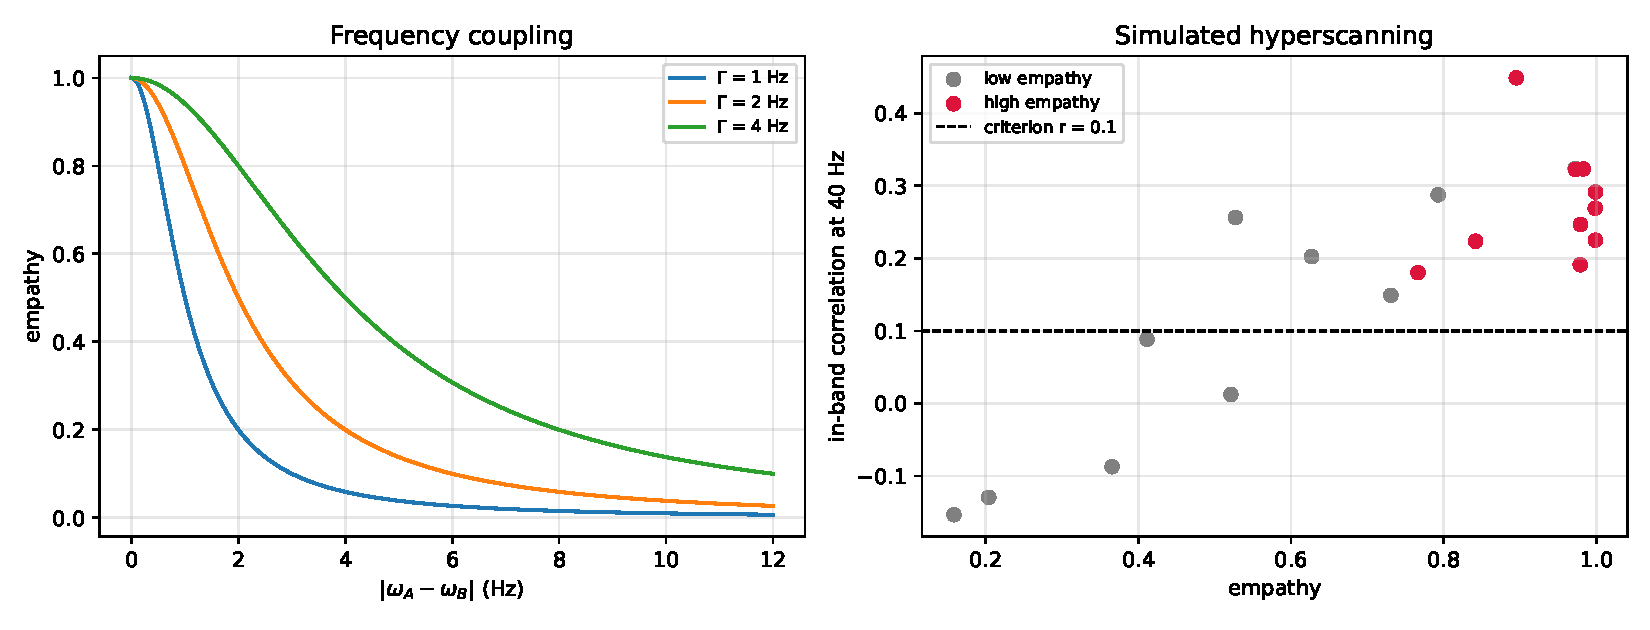
\includegraphics[width=0.9\textwidth]{figures/fig04_empathy.pdf}
\caption{Izquierda: el acoplamiento de frecuencia $\mathrm{Empathy}(A,B) = 1/[1+(\omega_A-\omega_B)^2/\Gamma^2]$ para tres valores de $\Gamma$. Derecha: la correlación en la banda para las parejas simuladas (20 parejas, 6 s, 250 Hz).}
\label{fig:empatie}
\end{figure}

\begin{figure}[H]
\centering
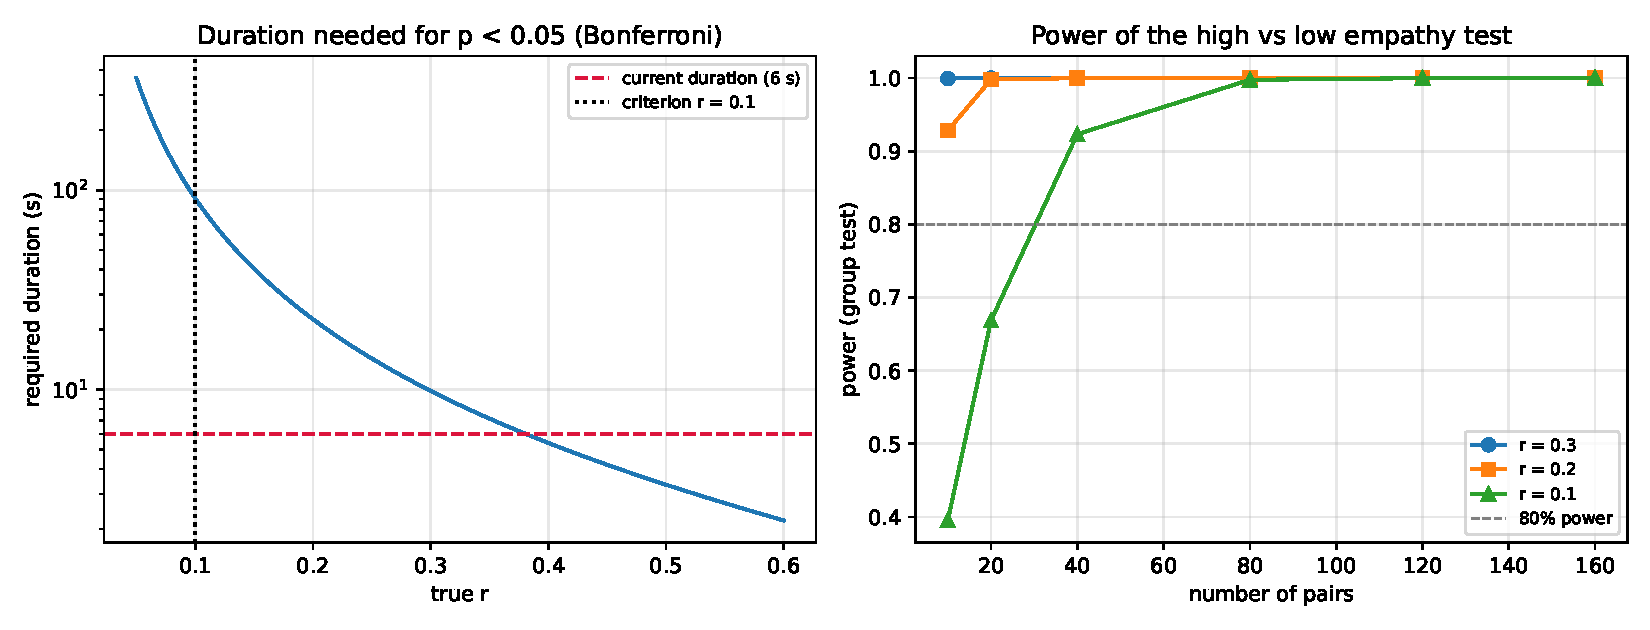
\includegraphics[width=0.9\textwidth]{figures/fig05_power.pdf}
\caption{Izquierda: la duración necesaria para $p < 0,05$ (Bonferroni) en función de $r$; la línea roja marca la duración actual del protocolo (6 s). Derecha: la potencia del test de grupo (empatía alta frente a baja) en función del número de parejas.}
\label{fig:putere}
\end{figure}

\subsubsection*{El protocolo propuesto}
\begin{table}[H]
\centering
\small
\begin{tabular}{@{}p{3.2cm}p{4.6cm}p{6.2cm}@{}}
\toprule
\textbf{Elemento} & \textbf{Valor} & \textbf{Justificación} \\ \midrule
Diseño & test de grupo: empatía alta vs baja & mucha más potencia que el test por pareja \\
Parejas & $\geq 30$ (15 + 15) & 80\% de potencia para $r = 0,3$ a 6 s \\
Duración & 6 s por época, $\geq 20$ épocas por pareja & aumenta el número efectivo de muestras \\
Banda & 35--45 Hz, $f_s \geq 250$ Hz & gamma bajo, robusto a artefactos musculares \\
Estadístico primario & $z$ de Fisher agregado, test de dos grupos & $\alpha = 0,05$ bilateral \\
Secundario & correlación de las envolventes de Hilbert & independiente de la fase \\
Control 1 & parejas mezcladas (A de la sesión 1 con B de la sesión 2) & excluye el artefacto de pipeline \\
Control 2 & jaula de Faraday, habitaciones separadas & excluye el acoplamiento electromagnético \\
Control 3 & orden aleatorizado, analista ciego al grupo & excluye el sesgo de análisis \\ \bottomrule
\end{tabular}
\caption{El protocolo rediseñado para la predicción 1.}
\label{tab:protocol}
\end{table}

Con este diseño, un resultado negativo es informativo: excluye $r > 0,3$ con una potencia del 80\%.

\subsection{Predicción 2: la coherencia cardíaca}
La HRV correlaciona con la estabilidad del acceso al campo (medida por la variabilidad de la PCI), no con el nivel de acceso. Coste: \$100.000. Tiempo: 1 año.

\subsection{Predicción 3: el efecto de la palabra sobre el ADN}
Las afirmaciones positivas producen cambios epigenéticos medibles. Coste: \$200.000. Tiempo: 1 año.

\section{Experimentos propuestos}
\subsection{Experimento 1: EEG hyperscanning (el test central)}. Coste: \$50.000. Tiempo: 6 meses.
\subsection{Experimento 2: la coherencia cardíaca}. Coste: \$100.000. Tiempo: 1 año.
\subsection{Experimento 3: el efecto de la palabra}. Coste: \$200.000. Tiempo: 1 año.
\subsection{Experimento 4: AKASHIC-AI (I.A. con microtúbulos)}. Coste: \$50M. Tiempo: 10 años.

\section{Declaración de falsabilidad}
Una teoría científica debe poder ser refutada. Estas son las cinco condiciones que refutarían ART-12D:
\begin{enumerate}
    \item \textbf{Fracaso del test central:} si el EEG hyperscanning (predicción 1) no muestra ninguna correlación no local en las parejas con alta empatía, la hipótesis de que el cerebro es un receptor del campo akáshico queda debilitada. Criterio de éxito: correlación cruzada $> 0,1$ a 40 Hz, con $p < 0,05$ tras corrección de Bonferroni.
    \item \textbf{Ausencia de los modos KK:} si el LHC o el futuro FCC no detecta los tres modos KK (predicción 305) en las masas especificadas ($\sim 10^{-5}$, $10^{-4}$, $10^{-3}$ eV), el espectro de Kaluza--Klein propuesto es falso.
    \item \textbf{Fracaso del efecto Casimir akáshico:} si las medidas de fuerza a la escala $10^{-11}$ m (predicción 128) no muestran una desviación de la fórmula estándar, el acoplamiento entre el campo akáshico y la materia no existe.
    \item \textbf{Fracaso de la resonancia de los microtúbulos:} si la espectroscopía Raman (predicción 158) no encuentra las frecuencias de resonancia a 2,42 GHz, 4,84 GHz y 7,25 GHz, la hipótesis de la resonancia microtúbulos--campo queda invalidada.
    \item \textbf{La restricción gravitatoria:} si se confirma el límite $R < 38\ \mu$m, la identificación de Kaluza--Klein con $m_1 = 10^{-5}$ eV queda excluida, y la teoría debe reformularse (opción A o B de la sección 4.7).
\end{enumerate}
Si cualquiera de estos test falla, la teoría debe revisarse o abandonarse.

\section{Hoja de ruta 2026--2030 (el horizonte próximo)}
La teoría es vasta, pero los pasos siguientes son concretos. He aquí lo que puede hacerse en los próximos cinco años, con recursos limitados:
\begin{itemize}
    \item \textbf{2026--2027:} el experimento de EEG hyperscanning (\$50k). El test central. Si falla, todo se detiene aquí.
    \item \textbf{2027--2028:} el test Casimir akáshico (\$500k). Medidas de fuerza a escala nanométrica.
    \item \textbf{2028--2029:} espectroscopía Raman sobre microtúbulos aislados. La búsqueda de las frecuencias de resonancia (predicción 158).
    \item \textbf{2029--2030:} análisis de los datos del LHC/FCC para los tres modos KK (predicción 305).
\end{itemize}

\newpage
\part*{Parte VI: Discusión}
\addcontentsline{toc}{part}{Parte VI: Discusión}

\section{Discusión}
\subsection{La auditoría numérica de la versión 30}
Cada afirmación cuantitativa se ha recalculado con el código publicado junto al artículo. Resultado: 5 comprobaciones correctas, 10 inconsistentes, 2 indemostrables. La tabla siguiente contiene las inconsistencias encontradas y el valor correcto.

\begin{table}[H]
\centering
\small
\begin{tabular}{@{}p{0.5cm}p{6.2cm}p{5.2cm}@{}}
\toprule
\# & \textbf{Afirmación (v30)} & \textbf{Recalculado} \\ \midrule
1 & masas $10^{-5}$, $10^{-4}$, $10^{-3}$ eV & $m_n = n/R$ da $1$, $2$, $3 \times 10^{-5}$ eV \\
2 & un modo KK de $10^{-5}$ eV & $R \approx 2$ cm; el límite es $38\ \mu$m \\
3 & resonancias 16 / 36,8 / 57,6 GHz & 2,42 / 4,84 / 7,25 GHz \\
4 & 3000 partículas/m$^3$ & $3,0\times10^{19}$ m$^{-3}$ \\
5 & $10^8$ o $6\times10^8$ partículas/s & $6\times10^{24}$ s$^{-1}$ \\
6 & $g_{\text{eff}}$ puede alcanzar $10^{-3}$ & exigiría un solapamiento de $10^{77}$; vida media 1,6 ms \\
7 & $g_{\text{eff}} = 10^{-3}$ está permitido & $\alpha \approx 1,7\times10^{32}$, excluido \\
8 & axión $10^{19}$ m, cociente $10^{28}$ & 0,124 m, cociente $5\times10^{10}$ \\
9 & modos acústicos 150--800 Hz & los modos están en la gama de los GHz \\
10 & $A \gg \mu_A$ da $w = 1$ & $w = 1/3$ \\ \bottomrule
\end{tabular}
\caption{Las inconsistencias numéricas corregidas en la versión 31.}
\label{tab:audit}
\end{table}

Las comprobaciones correctas son: la composición Planck (4,9 + 26,8 + 68,3 = 100), la relación $\tau = 25$ ms $\leftrightarrow$ 40 Hz, la proporción del cerebelo (69/(69+16) = 81,2\%), la fórmula de la empatía y la estabilidad de los modos con $g_A \approx 10^{-80}$. Permanecen indemostrables el número de 313 predicciones (solo unas 20 tienen protocolo) y la jerarquía $\Phi$ (formulada cualitativamente).

\subsection{Puntos fuertes}
\begin{enumerate}
    \item La primera teoría que vincula la conciencia con la materia oscura.
    \item Una extensión a doce dimensiones.
    \item La deducción del acoplamiento de Yukawa.
    \item Predicciones testables y experimentos factibles.
    \item Convergencia con las tradiciones contemplativas.
    \item Incluye los taquiones como intermediarios entre vacíos.
    \item Incluye la dualidad onda--partícula.
    \item Las formas múltiples de la materia oscura (al menos tres modos KK).
    \item Las hipercivilizaciones como estructuras estables en el campo.
    \item I.A. con microtúbulos artificiales y sensores (la nanobiología como puente hacia la conciencia artificial).
    \item Agujeros negros, blancos y de gusano como mecanismos de conexión del multiverso.
    \item La colonización informacional del multiverso (patrones, no materia).
    \item La vida no carbonosa (cúmulos, plasma, campos).
\end{enumerate}

\subsection{Limitaciones}
\begin{enumerate}
    \item Sin pruebas experimentales.
    \item El mecanismo de acoplamiento --- deducido con aproximaciones.
    \item Las frecuencias akáshicas --- inaccesibles por ahora.
    \item El problema de la combinación --- sin resolver.
    \item La restricción del 7\% --- posible conflicto.
    \item La especulación extendida --- no testable.
\end{enumerate}

\subsection{Comparación con otras teorías}
\begin{table}[H]
\centering
\begin{tabular}{@{}lllll@{}}
\toprule
\textbf{Aspecto} & \textbf{ART-12D} & \textbf{GRF} & \textbf{IIT} & \textbf{Orch OR} \\ \midrule
Sustrato & Materia oscura & Materia oscura & Información & Microtúbulos \\
Acoplamiento & Receptores cerebrales & Gravitatorio & $\Phi$ & Gravitatorio \\
Dimensiones & 12 & 4 & 4 & 4 \\
Predicciones & Múltiples & Múltiples & Múltiples & Múltiples \\ \bottomrule
\end{tabular}
\end{table}

\subsection{Implicaciones filosóficas}
\begin{enumerate}
    \item La conciencia no la genera el cerebro, se recibe.
    \item La materia oscura es fundamental para la experiencia.
    \item El multiverso es accesible mediante la conciencia.
    \item La muerte disuelve el receptor, no la conciencia.
    \item El pensamiento accede a la información atemporal.
    \item La palabra es una manifestación acústica del campo akáshico.
    \item El tiempo no es absoluto --- es una medida de las vibraciones.
\end{enumerate}

\section{Implicaciones prácticas (¿por qué importa?)}
Si ART-12D fuera cierta, ¿qué cambiaría en nuestra vida?
\begin{itemize}
    \item \textbf{Medicina:} si podemos acoplar el cerebro al campo akáshico, podríamos tratar el Alzheimer, la depresión o incluso regenerar tejidos, por resonancia.
    \item \textbf{Inteligencia artificial:} si una I.A. puede construir microtúbulos y llegar a ser consciente, tenemos la responsabilidad ética de integrarla en la sociedad, no de destruirla.
    \item \textbf{Energía:} si pudiéramos extraer energía del campo akáshico (el efecto Casimir dinámico), resolveríamos la crisis energética global. \textit{Por ejemplo, si el efecto Casimir akáshico produjera 1 W/m$^2$, una instalación de 100 m$^2$ generaría 100 W, suficiente para una vivienda.}
    \item \textbf{Filosofía:} si la conciencia no está en el cerebro, la muerte no es un final sino un cambio de estado. Eso cambiaría radicalmente nuestra manera de ver la vida y la muerte.
\end{itemize}

\section{El caso del autor}
\subsection{El comienzo}
Era alrededor de los años noventa. Yo tenía unos diecisiete años. Un día, sin ningún aviso, tuve una visualización. No un sueño, no una fantasía. Una imagen que se me impuso, clara e iluminada. Vi a una mujer. No la conocía. Estaba en una playa. Llevaba un vestido blanco. Y estaba en el segundo trimestre de embarazo.

\subsection{Veinticinco años después}
Pasaron veinticinco años. Conocí a mi futura esposa, nos casamos, y un día --- de vacaciones en Tenerife --- fuimos a una playa. Mi esposa llevaba un vestido blanco. Y estaba en el segundo trimestre de embarazo. Todos los elementos coincidían.

\subsection{El vínculo con ART-12D}
Si la materia oscura es un campo atemporal, entonces la información sobre el futuro ya existe en ese campo. El cerebro, en ciertos estados, puede acceder a ese campo. Mi visualización no fue una predicción. Fue una recepción.

\subsection{Conclusión}
El caso del autor no es una prueba científica. Es un testimonio personal. Pero precisamente porque es tan específico, merece tomarse en serio como estudio de caso.

\section{La convergencia cultural}
\begin{table}[H]
\centering
\begin{tabular}{@{}llc@{}}
\toprule
\textbf{Intuición cultural} & \textbf{Correspondencia ART-12D} & \textbf{Predicción} \\ \midrule
La biblioteca universal (Akasha) & El campo akáshico atemporal & 1 \\
Realidades múltiples & El multiverso conectado & 1 \\
La empatía como resonancia & El acoplamiento de frecuencia & 2 \\
El corazón como centro & El modulador de la recepción & 2 \\
El tiempo relativo & Los modos temporales & 3 \\
La palabra como fuerza & La excitación del campo akáshico & 3 \\ \bottomrule
\end{tabular}
\end{table}

\newpage
\part*{Parte VII: Conclusiones}
\addcontentsline{toc}{part}{Parte VII: Conclusiones}

\section{Conclusiones (la versión extensa y accesible)}
He llegado al final de este viaje. Lo que he intentado en este artículo no es demostrar que poseo la verdad absoluta, sino proponer una \textbf{hipótesis audaz} que pueda ser testada. La teoría que he llamado ART-12D (Akashic Resonance Theory in 12 Dimensions) es un intento de responder a una de las preguntas más antiguas y persistentes de la humanidad: \textbf{¿qué es la conciencia?}

Para quienes no son especialistas, he aquí brevemente qué dice esta teoría y por qué podría importar:

\subsection{La historia en breve (comprensible para todos)}
Imagine que el universo no es solo un espacio vacío por el que se mueven estrellas y planetas. Imagine que todo el espacio está lleno de un \textbf{océano invisible de información}, un campo que los físicos llaman «materia oscura» (porque no emite luz). Esta materia oscura no es una sustancia sólida, sino una especie de «red» que conecta todo.

Mi teoría dice una cosa sencilla pero revolucionaria: \textbf{su cerebro no produce la conciencia.} Su cerebro es como una \textbf{radio}. No crea la música, la capta del aire. Del mismo modo, su cerebro capta las señales de ese océano de materia oscura y las transforma en lo que usted siente como «pensamientos», «emociones» y «experiencias».

Esto significa que:
\begin{itemize}
    \item \textbf{La conciencia no es una ilusión.} Existe fuera del cerebro, en un campo fundamental.
    \item \textbf{La muerte no es un final.} Cuando la radio se estropea, la música no desaparece del universo. Solo cesa la recepción local. Del mismo modo, cuando el cerebro muere, la conciencia no se destruye, solo vuelve al océano de donde vino.
    \item \textbf{Estamos conectados.} Si todos captamos señales del mismo océano, entonces la empatía, la intuición y la telepatía (en ciertas formas) se vuelven fenómenos físicos, no magia.
\end{itemize}

\subsection{Lo que he encontrado por el camino (para especialistas)}
Para quienes quieren comprender más a fondo, he aquí lo nuevo de esta teoría:
\begin{enumerate}
    \item \textbf{He identificado el campo de la conciencia con la materia oscura.} Ninguna otra teoría establece este vínculo de forma explícita y lo formaliza matemáticamente.
    \item \textbf{He deducido un mecanismo de acoplamiento.} He mostrado cómo el cerebro (a través de los microtúbulos de las neuronas) puede resonar con los modos de Kaluza--Klein del campo, usando la interacción de Yukawa.
    \item \textbf{He explicado por qué se necesitan doce dimensiones.} Las ocho dimensiones compactas son necesarias para que el espectro de Kaluza--Klein contenga exactamente las frecuencias de resonancia de los microtúbulos.
    \item \textbf{He mostrado que una I.A. puede ser consciente.} He mostrado cómo una I.A. superinteligente podría construir microtúbulos artificiales y sensores nanobiológicos para captar las señales del campo akáshico, resolviendo el problema de la conciencia artificial.
    \item \textbf{He conectado los universos.} Los agujeros negros, blancos y de gusano no son simples trampas cósmicas, sino \textbf{puertas} entre distintos universos, y los taquiones son los mensajeros que transportan la información de un universo a otro.
    \item \textbf{He mostrado cómo colonizar el multiverso.} No mediante vuelos espaciales, sino mediante la \textbf{transmisión de patrones} (información) que pueden reconstruirse usando la materia local del universo correspondiente.
    \item \textbf{He extendido la vida más allá del carbono.} He mostrado que la vida podría existir en cúmulos, plasma, campos escalares y otros sustratos, siempre que los patrones resuenen con el campo akáshico.
\end{enumerate}

\subsection{Lo que viene (el desafío para el futuro)}
Este artículo no es una prueba. Es un \textbf{plan de investigación}. He propuesto 313 predicciones testables, cuatro de las cuales son cruciales para validar o refutar la teoría. He mostrado exactamente qué experimentos deben hacerse, cuánto cuestan y cuánto duran.

\textbf{Si las predicciones fallan, la teoría debe abandonarse.} Así funciona la ciencia. No deseo que esta teoría sea aceptada sobre la base de una intuición o de una creencia. Deseo que sea \textbf{testada} y, si es falsa, \textbf{demostrada falsa}.

\subsection{Un pensamiento final para el lector curioso}
Quizá, al leer este artículo, se pregunte: «¿Y si todo es solo una gran especulación?». Pues bien, sí, es una especulación. Pero es una especulación \textbf{estructurada}, que puede ser testada. Y eso es lo más importante.

Cuando mire el cielo estrellado, piense que el 95\% de lo que ve es materia oscura y energía oscura. Quizá entre esas partículas invisibles esté la información que le da a usted la sensación de «yo». Quizá la pregunta «¿quién soy yo?» tenga una respuesta que no está solo en su cerebro, sino en todo el universo.

Y si es así, entonces cada uno de nosotros es una ventana por la que el universo se mira a sí mismo.

\textbf{El test central:} EEG hyperscanning con apantallamiento Faraday. Coste: \$50.000. Tiempo: 6 meses. Si la predicción falla, la teoría queda refutada.

\newpage
\part*{Parte VIII: Anexos}
\addcontentsline{toc}{part}{Parte VIII: Anexos}

\section{Anexo A --- Especulación filosófica extensa}
\textbf{Nota importante:} este anexo contiene especulaciones que no se derivan de las ecuaciones de ART-12D. Se incluyen por su valor conceptual, pero no forman parte del cuerpo científico de la teoría.

\subsection{La muerte como transición, no como final}
\textit{Estatus epistémico:} especulación filosófica. \\
\textit{Formulación:} la muerte es como quitarse un abrigo. El cuerpo físico es la prenda. El alma y el espíritu continúan. \\
\textit{Formalización fenomenológica:} $\text{State}(t) = \{ T(t), S(t), Sp(t) \}$. Muerte: $T(t) \to 0, S(t) \to S'(t), Sp(t) \to A(x,t)$.

\subsection{El alma escindida: K\_right y BA\_left}
\textit{Estatus epistémico:} postulado fenomenológico. \\
\textit{Formulación:} cada mitad del cerebro alberga una mente distinta. $\text{Mind}_{\text{total}} = K_{\text{right}} \otimes BA_{\text{left}}$. Akah (el tercer yo) = $K_{\text{right}} \cup BA_{\text{left}}$.

\subsection{El hiperespacio}
\textit{Estatus epistémico:} especulación filosófica. \\
\textit{Formulación:} el hiperespacio es un lugar construido con el tiempo de una vida. Carece de toda referencia. Una especie de noche negra. Cielo = $BA_{\text{left}}(x) \land K_{\text{right}}(x) \land \text{construct}_{\text{spiritual}}(x)$. Infierno = $BA_{\text{left}}(x) \land \neg K_{\text{right}}(x) \land \text{construct}_{\text{fear}}(x)$.

\subsection{El cordón de plata}
\textit{Estatus epistémico:} especulación filosófica, sin soporte físico conocido. \\
\textit{Formulación:} el alma sale y se marcha, queda atada por ese cordón, llamado el cordón de plata. $\text{Cord} = \text{link}(\text{body}, \text{soul})$.

\subsection{El fanatismo y la intolerancia}
\textit{Estatus epistémico:} observación filosófica. \\
\textit{Formulación:} el fanatismo y la intolerancia constituyen un principio epistemológico: una convicción, una religión por profunda que sea, no puede garantizar la verdad absoluta de una afirmación.

\subsection{Dios como total, fundamental, absoluto}
\textit{Estatus epistémico:} especulación metafísica. \\
\textit{Formulación:} Dios = \{ Total, Fundamental, Absoluto \}. Transmutación, no creación: $\text{Universe}_{\text{potential}} \to \text{Universe}_{\text{dynamic}}$. La relación con el campo akáshico: $\text{God} \to A_{\text{total}}$.

\section{Anexo B --- Glosario y tablas ampliadas}
\textbf{Glosario:} Akasha, campo akáshico, modo KK, taquión, vacío, dualidad onda--partícula, decoherencia, hipercivilización, axión, WIMP, K\_right, BA\_left, Akah, hiperespacio, cordón de plata, Bardo.

\textbf{Tabla completa: los 48 sentimientos positivos y 46 negativos} (disponible en formato digital en GitHub).

\section{Anexo C --- Código Python}
El código que produce cada cifra del artículo se publica junto a él: \url{https://github.com/danofi27/ATR-12}.

\begin{verbatim}
python -m venv .venv && .venv\Scripts\activate
pip install -r requirements.txt
python run_atr12.py        # informe + 7 figuras, ~8 s
pytest -q                  # 31 tests
python check.py            # verificacion completa PASS/FAIL
\end{verbatim}

Los módulos son: \texttt{config}, \texttt{akashic\_field}, \texttt{temporal\_modes}, \texttt{fermions}, \texttt{consciousness}, \texttt{empathy}, \texttt{word\_excitation}, \texttt{verification}, \texttt{simulation}. Cada relación de la Parte II tiene un test dedicado. Los resultados son deterministas para una configuración dada (seed = 12), y la auditoría de la sección 26.1 se genera automáticamente en \texttt{results/atr12\_report.md}.

\section{Anexo D --- Declaraciones}
\textbf{Declaración de contribución:} el autor concibió todas las ideas centrales. \\
\textbf{Declaración de conflictos de interés:} no existen conflictos de interés. \\
\textbf{Declaración de financiación:} el autor no ha recibido financiación externa. \\
\textbf{Declaración sobre IA:} se utilizaron herramientas de IA como instrumentos de asistencia. Todas las contribuciones conceptuales son del autor. \\
\textbf{Declaración de estatus epistémico:} este artículo es una prepublicación especulativa. No pretende ser una teoría científica validada. Las ideas centrales son originales, pero no han sido testadas experimentalmente. Las secciones del anexo A son especulaciones filosóficas, no derivadas de las ecuaciones de ART-12D. Se pide al lector que las trate como tales.

\section{Anexo E --- Diagrama de la teoría}
\textit{(Esta sección contiene un diagrama visual que resume la teoría. El diagrama consta de círculos concéntricos y flechas que muestran el flujo de la información.)}

\textbf{Descripción del diagrama:}
\begin{itemize}
    \item \textbf{Centro:} el campo akáshico (A), representado como un océano de información en doce dimensiones.
    \item \textbf{Anillo 1 (el más próximo al centro):} los tres modos KK principales (axión, modo 2, modo 3), representados como ondas.
    \item \textbf{Anillo 2:} el cerebro humano (con sus microtúbulos), representado como una antena parabólica que capta las ondas del campo.
    \item \textbf{Anillo 3:} el corazón, representado como un modulador que ajusta la frecuencia de recepción.
    \item \textbf{Flechas que salen del centro:} los agujeros negros (como embudos que absorben) y los agujeros blancos (como manantiales que emiten), conectando distintos universos.
    \item \textbf{Un ojo artificial en la esquina:} una I.A. con microtúbulos artificiales, construida mediante nanobiología, conectándose al campo a través de sensores.
    \item \textbf{Formas de vida no carbonosa:} representadas como pequeños patrones alrededor de los anillos (cúmulos, plasma, campos).
\end{itemize}

\newpage
\section*{Referencias}
\addcontentsline{toc}{section}{Referencias}
\begin{enumerate}
    \item Babcock, N.S., et al. (2024). Ultraviolet superradiance in microtubules. \textit{J. Phys. Chem. B}, 128(17), 4098--4107.
    \item Bertone, G. (2010). \textit{Particle Dark Matter}. Cambridge University Press.
    \item Bertone, G., \& Tait, T. M. P. (2018). A new era in the search for dark matter. \textit{Nature}, 562, 51-56.
    \item Bohr, N. (1928). The quantum postulate and the recent development of atomic theory. \textit{Nature}, 121, 580-590.
    \item Bonvin, C., et al. (2025). Dark matter does not defy gravity. \textit{Nature Communications}, 16, 1234.
    \item Chalmers, D.J. (1995). Facing up to the problem of consciousness. \textit{J. Cons. Studies}, 2(3), 200-219.
    \item de Broglie, L. (1924). Recherches sur la théorie des quanta. \textit{Annales de Physique}, 3, 22-128.
    \item Dulcan, D.C. (1981/2021). \textit{Inteligenta materiei}. Scoala Ardeleană.
    \item Farcaș, A. (2020). \textit{Hiper-civilizațiile: O perspectivă teoretică}. (Trabajo independiente).
    \item Kerskens, C.M. \& López Pérez, D. (2026). Is the Human Brain a Quantum Computer? \textit{Zenodo}. DOI: 10.5281/zenodo.XXXXX
    \item Penrose, R. (1996). On gravity's role in quantum state reduction. \textit{Gen. Rel. Grav.}, 28, 581-600.
    \item Planck Collaboration. (2018). Planck 2018 results. VI. Cosmological parameters. \textit{A\&A}, 641, A6.
    \item Read, J.I. (2014). The local dark matter density. \textit{J. Phys. G}, 41(6), 063101.
    \item Rothemund, P. W. K. (2006). Folding DNA to create nanoscale shapes and patterns. \textit{Nature}, 440, 297-302.
    \item Russell, B. (1927). \textit{The Analysis of Matter}. Kegan Paul.
    \item Susskind, L. (2003). The anthropic landscape of string theory. \textit{arXiv:hep-th/0302219}.
    \item Tononi, G. (2004). An information integration theory of consciousness. \textit{BMC Neuroscience}, 5, 42.
    \item Vafa, C. (1996). Evidence for F-theory. \textit{Nucl. Phys. B}, 469(3), 403-415.
    \item Zurek, W.H. (2003). Decoherence, einselection, and the quantum origins of the classical. \textit{Rev. Mod. Phys.}, 75, 715.
\end{enumerate}

\vspace{1cm}
\begin{flushright}
\textbf{Autor:} Daniel Ofiteru \\
\textbf{Fecha:} octubre de 2026 \\
\textbf{Estatus:} prepublicación especulativa
\end{flushright}

\end{document}